
\hide{%%%%%%%%%%%%=================================================================
\section{Problem}

We formalize the problem of graph-based anomaly detection. 
%\subsection{Graph-based Anomaly Detection Problem}
We denote a graph as $G = \left(V, X, A\right)$, where 
$V$ is the set of $N$ nodes, 
$A \in \mathbb{R}^{N \times N}$ denotes the adjacency matrix, 
and ${X}$ is the corresponding feature vectors with $\boldsymbol{x}_i \in \mathbb{R}^d$ denoting the $d$-dimensional feature vector of $v_i \in V$. 
%Generally, $A$ can carry arbitrary edge features to represent various graph properties such as the unweighted or weighted, the undirected or directed, and the single-relational or multi-relational graphs. 
Without loss of generality, 
%To generalize to various scenarios of anomaly detection, 
we consider $G$ into an unweighted, undirected, and single-relational graph, i.e., $A_{ij} = 1$ if there exists an edge between $v_i$ and $v_j$ and $A_{ij} = 0$ otherwise.

\begin{problem}
	
	\textbf{Anomaly Detection with Graphs.} 
	Given a labeled graph $G = \left(V, X, A, Y\right)$, $Y$ is the set of labels on nodes with $y_i \in Y$ takes value 1 if $v_i$ is abnormal and 0 otherwise. 
%	The goal is to learn a predictive function $f: V \rightarrow \mathbb{R}^d$ that maps each node into a $d$-dimensional space ($d \ll |V|$). 
	%The function $f$ needs to preserve both the structural information and the input features of the nodes. 
	The goal is to learn a classifier $g: \mathbb{R}^d \rightarrow \{0,1\}$ to determine whether a given node is abnormal (1) or normal (0). 
\end{problem}

To address this problem, most existing studies focus on explicit structural engineering~\cite{}. \yx{add >=3 old kdd}
In this work, we instead to leverage contrastive learning and graph neural networks (GNNs) for modeling the structural anomalies. 


}%end of hide%%%%%%%%%%%%%=================================================================


%\subsection{The \smodel Model}

\section{\model}
\label{sec:approach}
% We present \model, the graph contrastive coding model, 
In this section, we first introduce the problem definition of anomaly detection (\secref{sec:problem}), and then conduct the preliminary observations to verify the motivation of \smodel(\secref{sec:problem}). After that, we propose the  learning objective with theoretical guarantees (\secref{subsec:overview}), and further extend the supervised objective to the unsupervised setting (\secref{subsec:self}). 
Finally, we introduce the context-aware GNN encoder of \smodel and \spmodel(\secref{subsec:gnn}).




\subsection{The Studied Problem}
\label{sec:problem}
% We formalize the problem of graph-based anomaly detection. 
%\subsection{Graph-based Anomaly Detection Problem}
We define a graph as $G = \left(V, X, A, Y\right)$, where 
$V$ is the set of $N$ nodes, 
$A \in \mathbb{R}^{N \times N}$ denotes the adjacency matrix,
and ${X} \in \mathbb{R}^{N \times d}$ is the corresponding feature vectors with $\boldsymbol{x}_i \in \mathbb{R}^d$ representing the $d$-dimensional feature vector of node $v_i$.
%Generally, $A$ can carry arbitrary edge features to represent various graph properties such as the unweighted or weighted, the undirected or directed, and the single-relational or multi-relational graphs. 
Without loss of generality, 
%To generalize to various scenarios of anomaly detection, 
we consider $G$ as an undirected and single-relational graph, i.e., $A_{ij}\, \textgreater\, 0$ if there exists an edge between $v_i$ and $v_j$ and $A_{ij} = 0$ otherwise.

\begin{problem} \textbf{Graph-based Anomaly Detection.} Given a graph $G = \left(V, X, A, Y\right)$, $Y$ is the set of node labels with $y_i \in Y$ equals to 1 if $v_i$ is abnormal and 0 otherwise. 
%	The goal is to learn a predictive function $f: V \rightarrow \mathbb{R}^d$ that maps each node into a $d$-dimensional space ($d \ll |V|$). 
	%The function $f$ needs to preserve both the structural information and the input features of the nodes. 
	The goal is to learn a function $g: \mathbb{R}^d \rightarrow \{0,1\}$ to determine whether a given node is abnormal (1) or normal (0). 
\end{problem}

To resolve this problem, most existing GNN-based models directly instantiate $g$ as a binary classifier~\cite{dou2020enhancing,liu2020alleviating}. 
We conduct the following preliminary observations to verify the motivation of the proposed model.
%Inspired by the observations about the distinguished distances to the global context (Figure~\ref{fig:para}), we instead leverage contrastive learning for detecting the anomalies. 


\begin{figure}[t]
	\centering
	\hspace{-0.1in}
	%\subfigure[AMiner]{\label{subfig:paper_network}
	%	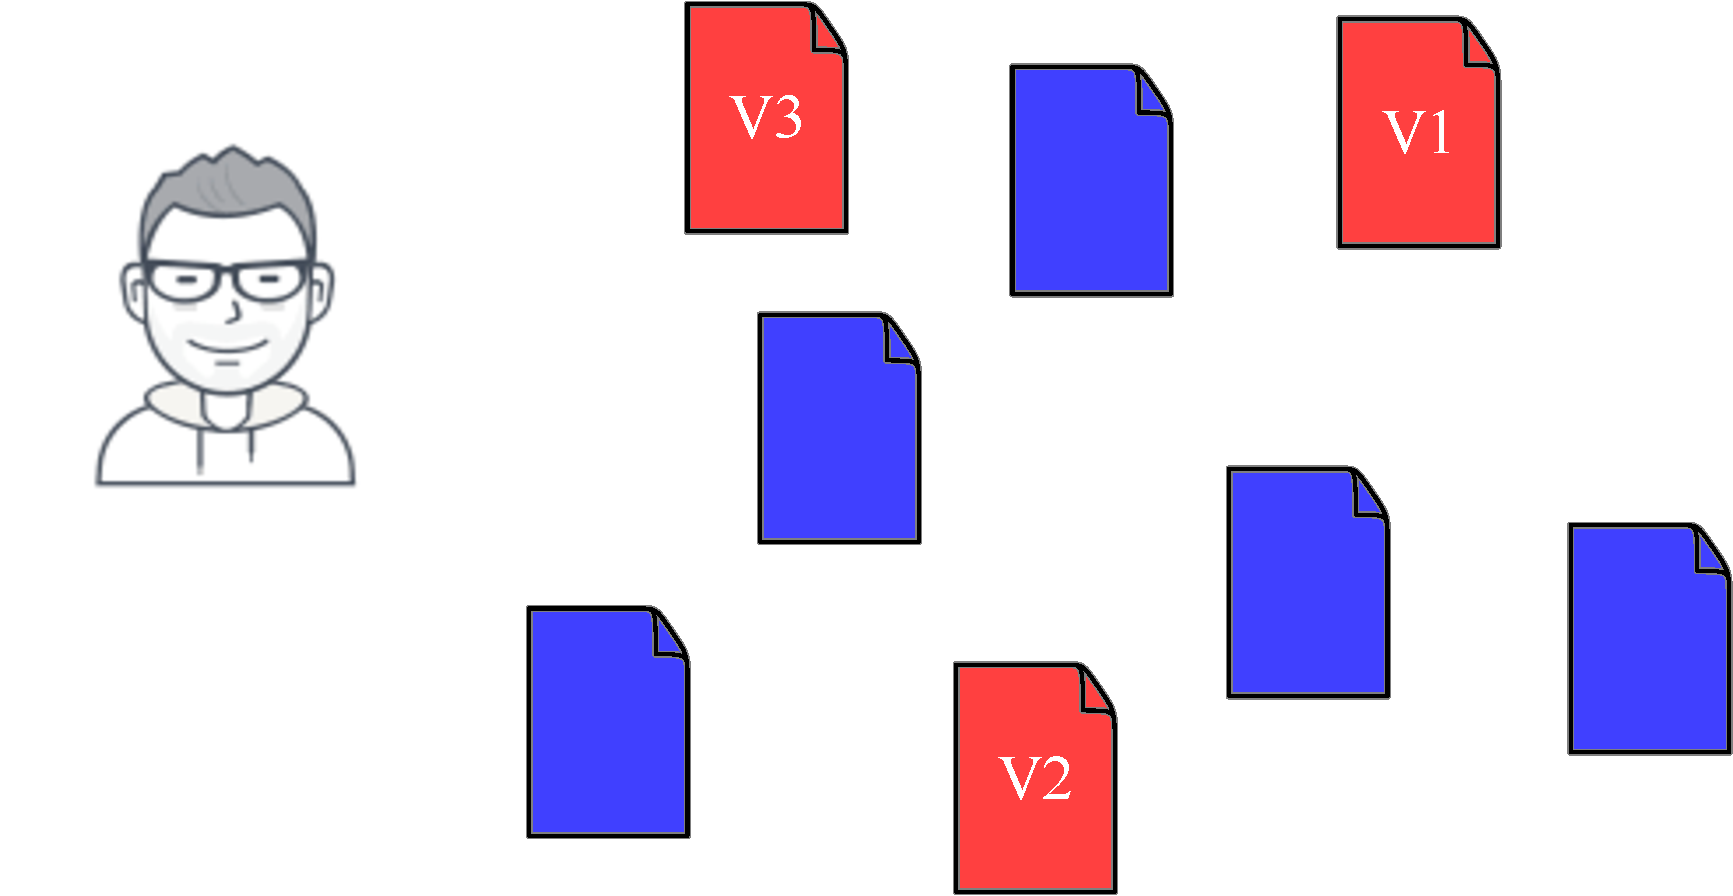
\includegraphics[width=0.33\textwidth]{figures/motivation}
	%}
	%\subfigure[t-SNE]{\label{subfig:t-sne}
	%	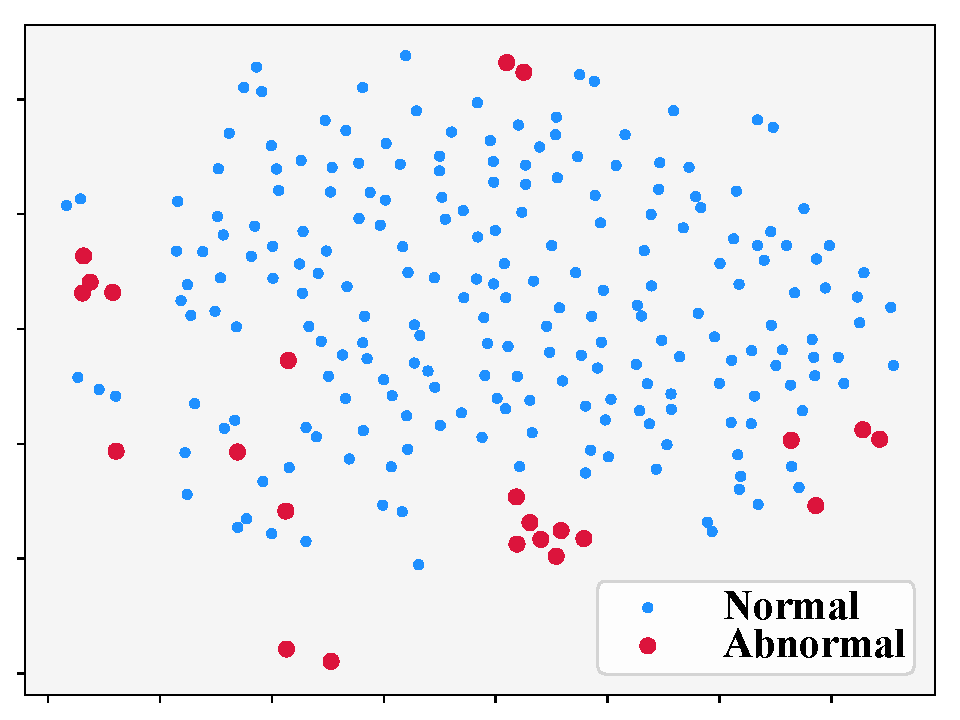
\includegraphics[width=0.19\textwidth,  height=0.11\textheight]{figures/diverse_tsne}
	%}
%\hspace{-0.15in}
	\subfigure[Input Feature (Distribution)]{\label{subfig:class_pro}
		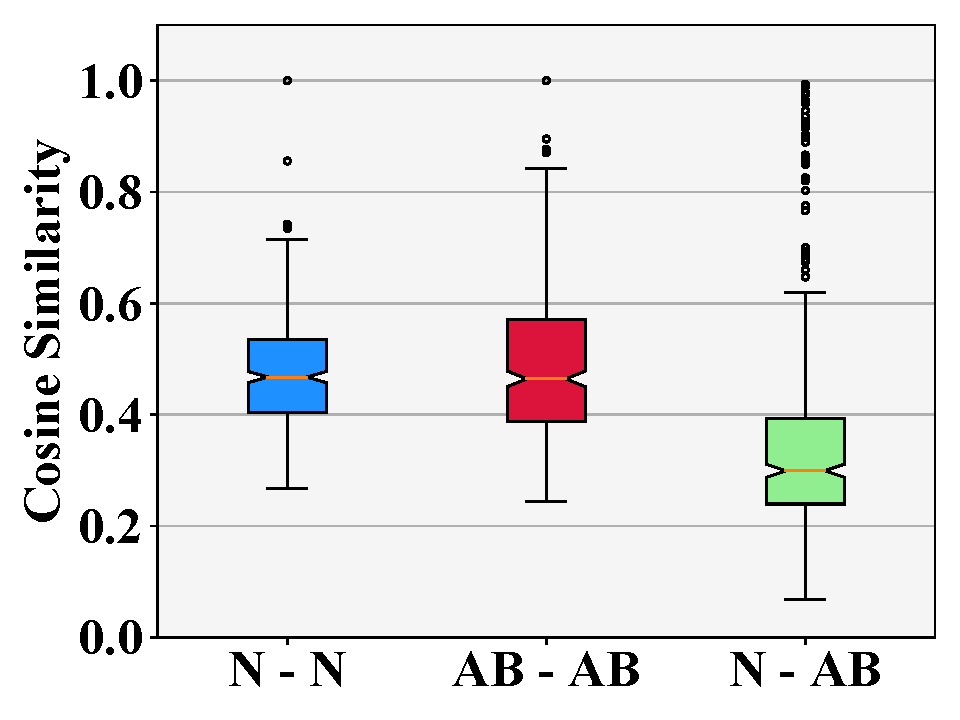
\includegraphics[width=0.22\textwidth]{figures/observe_classifier_pro}
	}
%\hspace{-0.15in}
	\subfigure[Embeddings by GCN]{\label{subfig:class_after}
	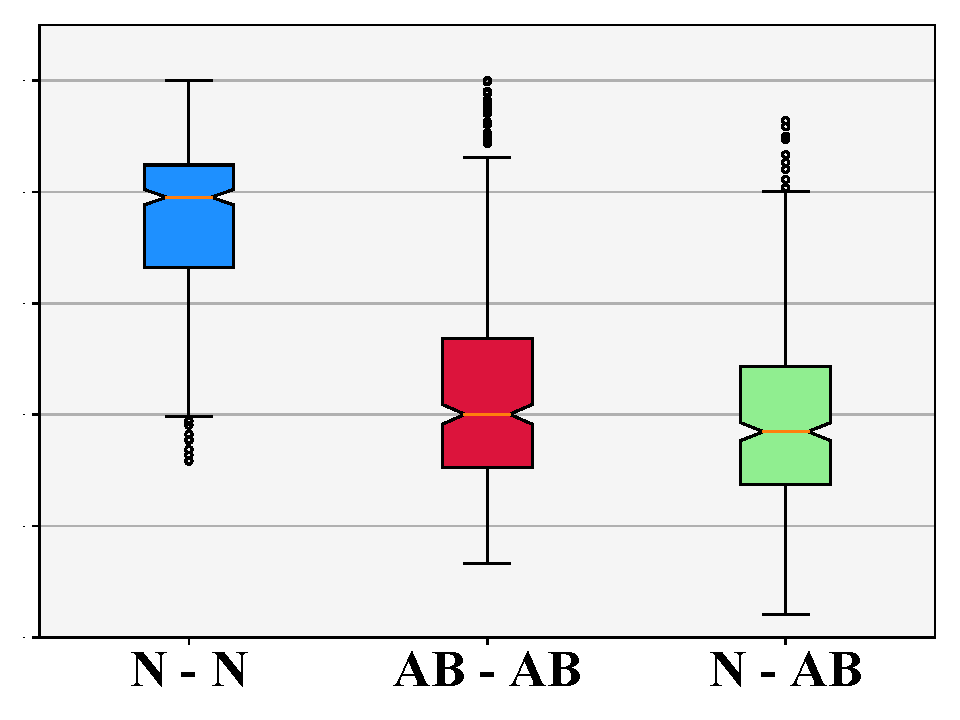
\includegraphics[width=0.21\textwidth,  height=0.121\textheight]{figures/obs_classifier_after}
}
%\hspace{-0.15in}
	\subfigure[Input Feature (Global Cons.)]{\label{subfig:con_pro}
		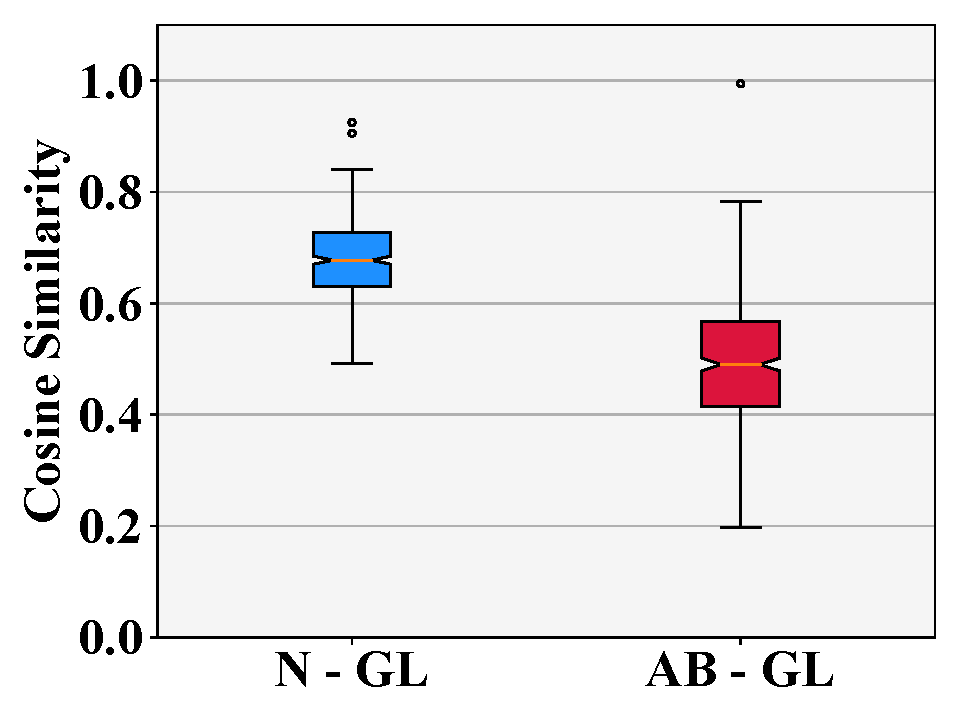
\includegraphics[width=0.22\textwidth]{figures/obs_con_before}
	}
%\hspace{-0.15in}
	\subfigure[Embeddings by \model]{\label{subfig:con_after}
	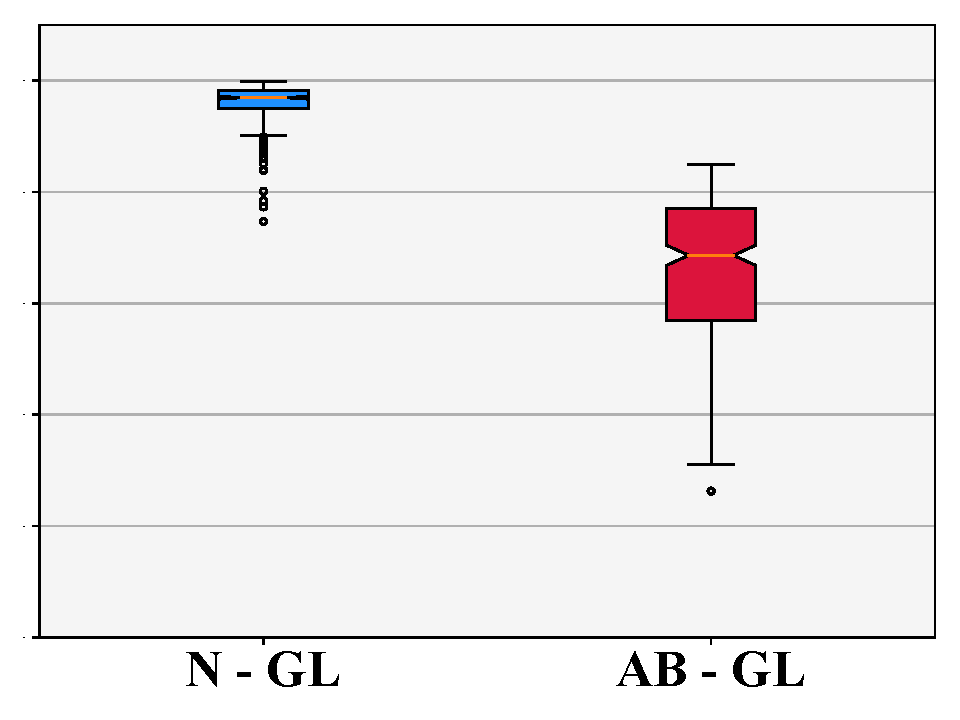
\includegraphics[width=0.21\textwidth,  height=0.121\textheight]{figures/obs_con_after}
	}

	\caption{\label{fig:obervation}  %, a professor from University of Munich. 
		%(a) The t-SNE projection of the graph of all his papers, wherein nodes are papers and if two papers share the same coauthors or venues, an edge links them; 
		(a) The similarities between normal and normal nodes (blue), abnormal and abnormal nodes (red), and normal and abnormal nodes (green) by the BERT-initialized input features; 
		%(N and AB are abbreviated for \underline{N}ormal nodes and \underline{AB}normal nodes respectively);
		(b) The similarities between embeddings generated by GCN.
		(c) The similarities between normal nodes and the global context (blue) vs. those between abnormal nodes and the global context (red) by the input features;
		%(GL is abbreviated for \underline{GL}obal context); 
		(d) The similarities between embeddings generated by \model.}  
\end{figure}


\vpara{Preliminary Observations.} To further verify the motivation of contrasting a node with the global context in Fig.~\ref{fig:para}, we additionally extract 10,000 authors owning more than 500,000 papers from AMiner\footnote{https://www.aminer.org/}. Each author profile is treated as a graph with its papers as nodes and connections among papers as edges.
% a free online academic search and mining system. 
Notably, we mainly focus on detecting anomalies in the multi-graph setting in this paper, which is a more challenging and under-explored scenario (Cf. Section 3.2). 
% Thus, here we mainly discuss related cases based on the multi-graph datasets, e.g., AMiner. 
However, our proposed method can also be instantiated as the single-graph setting.
Likewise, the goal here is to detect the wrongly assigned papers (anomalies). For each author, the wrongly assigned papers (anomalies) are labeled by professional annotators or the author themselves. For each paper, we obtain its BERT embedding~\cite{devlin2019bert} by its title. Then we calculate the cosine similarity between a pair of papers and average the pairwise cosine similarities of three groups, i.e.,  \underline{N}ormal and \underline{N}ormal (N-N), \underline{AB}normal and \underline{AB}normal (AB-AB), and \underline{N}ormal and \underline{AB}normal (N-AB). 
Fig.~\ref{subfig:class_pro} shows the following phenomenon.
\begin{itemize}
	\item \textbf{Intra-Diversity:} The similarities in both N-N and AB-AB are extremely diverse (being scattered within [0.2,0.8]), which is in concert with the case in Fig.~\ref{subfig:t-sne}; 
	\item \textbf{Inter-Diversity:} The similarities of N-AB are also diverse, and more than 20\% abnormal nodes are similar to the normal nodes (y $>$ 0.5).
\end{itemize}


%We can see that the similarities distributions in both \textit{N-N} and \textit{AB-AB} are extremely %diverse (Scatter evenly between 0.2 and 1.0). Moreover, from the similarity distribution of %\textit{N-AB}, we find that more than 20\% abnormal nodes are similar with normal nodes (y $>$ 0.5), 

We conjecture this intra-/inter- diversity will degrade the performance of distinguishing anomalies from normal ones by the traditional classifier. To verify this, we investigate the same similarities based on the embeddings generated by GCNs~\cite{kipf2016semi} with the binary classification loss, as shown in 
Fig.~\ref{subfig:class_after}. It demonstrates that although the similarities in N-N increase from [0.2, 0.8] to [0.4, 1.0], the intra- and inter- diversity issues are still severe. 
% which can be attributed into two perspectives: 1) The violation of class-homophily assumption catastrophically degrades the representation capability of GNNs,
% and
% 2) The intrinsic diversity shown in Figure~\ref{subfig:class_pro} incapacitate the classifiers to directly separate the abnormal nodes from normal ones. 
%which empirically implies that resolve the anomaly detection problem in a binary classification fashion may not always be the silver bullets for all the scenarios.

Previous efforts~\cite{liu2020alleviating, kumar2018rev2} disclose the behavior patterns of anomalies are different from those of normal nodes, based on which they characterize the inductive bias to detect anomalies. 
However, most of them only focus on modifying the message passing process to reduce propagated noises, while ignoring the limited capability of the binary classification objective 
when the data distribution is diverse. 
% (Fig.~\ref{subfig:class_pro},~\ref{subfig:class_after}). 
% As the default setting of anomaly detection is the normal nodes are the majority of a whole graph, the behavior pattern deviations between abnormal and normal nodes can further be viewed as that between abnormal nodes and the global context of a graph. 

Inspired by the case observed in Fig.~\ref{subfig:similarity}, we compute the similarity between each node and the global context---the average of all the node features\footnote{The global context is later estimated by the memory-based context updater.}, and show the average similarities in N-GL and AB-GL in Fig.~\ref{subfig:con_pro}. 
We can see that, compared with Fig.~\ref{subfig:class_pro}, although still having overlaps, the two similarity distributions can be distinguished much more clearly. 
% Furthermore, the similarities based on the embeddings of the normal and abnormal ones generated by the proposed \smodel, shown in Fig.~\ref{subfig:con_after}, can be further distinguished compared with Fig.~\ref{subfig:con_pro}.
Furthermore, we plot the similarities based on the embeddings generated by \smodel in Fig.~\ref{subfig:con_after}. Compared with Fig.~\ref{subfig:con_pro}, the resultant embeddings of normal and abnormal ones can be further distinguished.  

To this, we empirically verify the motivation of the context-aware contrastive learning method --- instead of directly capturing the absolute difference between normal and abnormal nodes, contrasting the relative distances between the node and global context is expected to be a more promising way to address the diversity of node distributions. 



%\subsection{Context-aware Graph Contrastive Learning}
% \subsection{The \smodel Model}
\subsection{Methodology}
\label{subsec:overview}
%Existing GNN-based methods instantiate $f$ as a GNN encoder (i.e., $f_{\text{GNN}}$) and $g$ as a discriminative layer such as MLP, to directly map a node embedding into a binary value~\cite{dou2020enhancing,liu2020alleviating}. 

%However, anomaly detection cannot be simply treated as a general binary classification problem, because the abnormal nodes as well as the normal nodes present diverse feature distributions, which makes it challenging to find a clear boundary by binary classification. 

%For example, in Figure 1, for cleaning the researcher's profiles, the wrong papers denoted by red nodes distinguish from the normal pattern in various aspects, i.e., the features of wrong papers are not consistent. 

%Similarly, for detecting the fraudsters who publish malicious comments on products in business websites, the fraudsters may comment on different kinds of products. 
%Simultaneously, the normal nodes may also present diverse patterns due to diverse preferences. 
%For example,  a researcher may publish papers in multiple topics with different groups of coauthors in various venues, resulting in a diverse paper network. Similarly, the abnormal users in business websites may favour different categories of products. 
%Such diverse features of the abnormal and the normal nodes will hurt the performance of node binary classification.
%Despite the irregular node features, we discover the difference of the distance to the global context between the normal nodes and the abnormal nodes; that is, the anomalous extent of a node depends more on its deviation from the majority of the nodes than its own features.


The basic idea of \smodel is to determine a node's abnormality by contrasting it with the global context of the entire graph. 
This is motivated by the discovery that there exists a significant difference in the distance to the global context between normal and abnormal nodes. In another words, a node is more abnormal if it deviates farther away from the majority of nodes in the feature space. 
%the anomalous exhibit large deviations from the majority of the nodes than its own features. 
%The underlying assumption is a node is more abnormal if it deviates farther away from the whole context. 

In view of this, we distinguish abnormal and normal nodes in the embedding space by the graph contrastive learning (\model).
%\underline{Co}ntext-aware \underline{G}raph \underline{C}ontrastive \underline{L}earning (\model). 
%with a context-aware graph contrastive objective function. % instead of the binary classification objective function. 
Specifically, given a graph ${G}$, we first create a GNN encoder $f_{\text{GNN}}$ that can output an embedding $\boldsymbol{h}_i$ for each node $v_i$ and also an embedding $\boldsymbol{q}$ for the entire graph (global context), i.e., (${H}, \boldsymbol{q}) = f_{\text{GNN}}({X}, {A}, {W})$ with $H = \{\boldsymbol{h}_i\}_{i=1}^{N}$ and $W$ as the trainable parameters of $f_{\text{GNN}}$. 
We take the graph embedding $\boldsymbol{q}$ as the query, a normal node's embedding as the positive key that matches with $\boldsymbol{q}$, and the embeddings of all the abnormal nodes as the negative keys that don't match with $\boldsymbol{q}$. 
For implementation, we use infoNCE~\cite{oord2018representation} in a \textit{supervised} manner 
%---a well-adopted loss function in contrastive learning---
as the concrete loss function such that:

\beq{
	\label{eq:loss}
	\mathcal{L}_{\text{con}} \!=\!\!\!\! \mathop{\mathbb{E}}\limits_{i: y_i = 0 \atop j:y_j=1}\!\!\left[\!-\!\log \frac{\exp \left(\textbf{q}^\top\boldsymbol{h}_i/\tau\right)}{ \sum_{ j} \exp \left(\boldsymbol{q}^\top \boldsymbol{h}_j/\tau\right) + \exp \left(\boldsymbol{q}^\top\boldsymbol{h}_i/\tau\right) }\!\right]
}

\noindent where $\tau$ is the temperature hyperparameter. The objective function is to enforce maximizing the consistency between the positive pairs (normal node, global context) compared with negative pairs (abnormal node, global context). 

Compared with the context-aware contrastive learning, the traditional normal-abnormal contrast is a node-wise contrastive pattern, which usually suffers from noisy labels. For example, \cite{kalantidis2020hard} states that false-negative instances hinder the performance of contrastive learning. On the contrary, the proposed local-global method contrasts each abnormal node with the global context, which can reduce the negative influence of individual noisy labeled nodes. 


\vpara{Why does \smodel work?}
%Fundamentally, the bottleneck of anomaly detection is to differentiate the abnormal behavior patterns from normal ones. Inspired by Quantitative Observations aforementioned, we instead to optimize the relative distance between nodes and global context, rather than charactering the absolute distribution gap between abnormal and normal nodes. 
%We now provide two theoretical guarantees to confirm the efficacy of global context contrastive objective,
%We now provide a theoretical guarantee to confirm the efficacy of global context contrastive objective. 
We theoretically prove the effectiveness of the proposed \smodel compared with the original cross-entropy loss for classification.

% \begin{theorem} 
% \textit{Minimizing the contrastive loss in Eq. \eqref{eq:loss} forms the lower bound of: 
% 		1) Kullback-Leibler (KL) divergence between the abnormal and normal node distribution, 
% 		and, 
% 		2) the entropy of abnormal node distribution. }
		
% 	Let $p_{\text{nor}}(\cdot)$ be the data distribution over $\mathbb{R}^d$ of normal node embedding and $H^+ = \{\boldsymbol{h}^+_i\}_{i=1}^{n}$ is the normal node embedding matrix with the length $n$. 
% 	Likewise, we define corresponding  $p_{\text{abnor}}(\cdot)$ and $H^- = \{\boldsymbol{h}^-_i\}_{i=1}^{m}$ of abnormal nodes. We set $n\!\gg\! m$, and claim $p_{\text{abnor}}(\cdot)$ and $p_{\text{abnor}}(\cdot)$ are mutually independent, which agree with the canonical setting of anomaly detection.
% 	$\mathcal{R}(\cdot)$ be a deterministic readout function on graphs, without loss of generality, assume $\mathcal{R}(\cdot) = \text{MEAN}(\cdot)$ be the geometric average operation, such that $\boldsymbol{q} = \mathcal{R}(H) = \frac{1}{N}(\sum_{i=1}^{n}\boldsymbol{h}^+_i + \sum_{j=1}^{m}\boldsymbol{h}^-_j)$. 
% 	Then we have:
%     \beq{
%     \min\limits{w}\text{Eq.}~\eqref{eq:loss} \triangleq \max \left[\hat{D}_{KL}(\boldsymbol{h}^-||\boldsymbol{h}^+) + 2\hat{H}(\boldsymbol{h}^-)\right] 
%     }
% % 	Then we have: \textit{minimizing the contrastive loss in Eq. \eqref{eq:loss} forms the lower bound of: 
% % 		1) Kullback-Leibler (KL) divergence of the two data distributions, $p_{\text{nor}}(\cdot)$ and $p_{\text{abnor}}(\cdot)$, 
% % 		and, 
% % 		2) the entropy of $p_{\text{abnor}}(\cdot)$. 
% % 	}  
% \end{theorem}
% % \zj{dimension size is d rather than n, node number is  N rather than n. It may be better to first give the theorem and then explain the two distributions and the corresponding notations.}


\begin{theorem} 
	Let $X^+$\footnote{We denote random variables using upper-case letters (e.g. $X^+$, $X^-$ ), and their realizations by the corresponding lower-case letter (e.g. $x^+$, $x^-$).} denote the random variable of normal node and $p^+(\cdot)$ denote its marginal distribution, thus $X^+\!\sim \!p^+(x^+)$. Likewise, we denote the abnormal node by $X^-$ and its marginal distribution by $p^-(\cdot)$, $X^-\!\sim \!p^-(x^-)$. Assume $p^+$ and $p^-$ are mutually independent.
	Then we have: \textit{minimizing the contrastive loss in Eq. \eqref{eq:loss} forms the lower bound of 
		1) the cross-entropy of the two data distributions $p^+(\cdot)$ and $p^-(\cdot)$ plus 
		2) the entropy of $p^-(\cdot)$.} Formally,  

    \beq{
    \label{eq:theory}
    \min \mathcal{L}_{\text{con}} \triangleq \max \left[H(p^-||p^+) + H(p^-)\right].
    }
\end{theorem}



In view of the two parts in Eq.~\eqref{eq:theory}, the contrastive loss $\mathcal{L}_{\text{con}}$ is theoretically and analytically more robust than the cross-entropy loss and node-wise contrastive loss because of the following reasons.


First, the local-global contrast can better deal with the diverse abnormal distribution. Theorem 1 shows that the proposed local-global contrastive loss can be decomposed into the cross-entropy between the distribution of the normal node and the abnormal node plus the entropy of the abnormal node. Since the first term links to the node-wise contrastive loss~\cite{boudiaf2020unifying}, which is also proved to be the cross-entropy between the predicted labels and the ground truth labels~\cite{boudiaf2020unifying}, the proposed local-global contrastive loss has an additional entropy of the abnormal node compared with the cross-entropy loss. Such additional entropy, acting as a normalization constraint, makes the distribution of learned abnormal node features spread uniformly as much as possible in the feature space. 
Thus it can better deal with the diverse feature distributions, especially the abnormal diverse distribution, which can be exactly observed in the anomaly detection datasets (Cf. Fig.~\ref{fig:para}). 


Second, the local-global contrast can reduce the label-imbalance issue. Maximizing the additional entropy of abnormal nodes also augments informative features of the abnormal nodes, reducing the label imbalance issue of the abnormal nodes against the normal nodes to some degree. The common assumption in anomaly detection is that the abnormal node is the minority class, because the number of abnormal nodes is much smaller than normal ones. Thus, traditional anomaly detection methods usually suffer from the class imbalance issue. To alleviate it, data augmentation techniques for generating pseudo-labels of the minority classes [3], up-sampling or down-sampling techniques for re-balancing the class distribution [4], etc., are proposed. The core insight is to augment the information of minority classes, which can balance the training bias between majority classes and minority classes. Such the balancing technique somehow agrees with the optimizing goal of the second part of Eq.~\eqref{eq:theory}, which augments informative features of the abnormal nodes to balance the training bias.
                                          


% \vpara{Connection to Cross Entropy.}  Although Cross Entropy loss is equivalent to KL divergence when facing fixed target distributions, $p_{\text{abnor}}(\cdot)$ is a unknown deterministic factor condition on different scenarios (especially with multi-graph datasets in \secref{sec:exp}), KL divergence here is more resilient than Cross Entropy when encountering dynamic node distributions.

% \ipara{Connection to Class Imbalance.} Class imbalance is the Achilles' heel of the anomaly detection problem. Many efforts devoted to adopt self-supervised learning to augment and preserve the information of minority classes~\cite{wei2021crest, yang2020rethinking}, which is in concert with maximizing the entropy of abnormal distribution $H(\boldsymbol{h}^-)$.   
%\end{itemize}


\vpara{Proof of Eq.~\eqref{eq:theory}.} 
Let $\boldsymbol{h}^+$ = $f_{\text{GNN}}\left(x^+, \cdot, W\right)$, where $\boldsymbol{h}^+_i \in \mathbb{R}^d$, then we have the normal node embedding matrix $H^+ = \{\boldsymbol{h}^+_i\}_{i=1}^{n}$, where $n$ is the number of normal nodes. Likewise, we define $\boldsymbol{h}^-$ = $f_{\text{GNN}}\left(x^-, \cdot, W\right)$ and the abnormal node embedding matrix $H^- = \{\boldsymbol{h}^-_j\}_{j=1}^{m}$ with the node number $m$. Note that, $n\!\gg\! m$.
Let $\mathcal{R}(\cdot)$ be a deterministic readout function on graphs. Without loss of generality, we assume $\mathcal{R}(\cdot) = \text{MEAN}(\cdot)$. Thus $\boldsymbol{q} = \mathcal{R}(H) = \frac{1}{N}(\sum_{i=1}^{n}\boldsymbol{h}^+_i + \sum_{j=1}^{m}\boldsymbol{h}^-_j)$. 
From Eq.~\eqref{eq:loss}, we can derive

\begin{small}
\beqn{
\label{eq:lossf}
 \mathcal{L}_{\text{con}} &=& 
\underbrace{\mathop{\mathbb{E}}\limits_{x^+\sim p_{\text{n}}}\left[-\boldsymbol{q}^T\boldsymbol{h}^+/\tau\right]}_{\text{alignment}} \\ \nonumber
&+& \!\!\!\!\!\!\underbrace{\mathop{\mathbb{E}}\limits_{x^+\sim p_{\text{n}},\atop \{x^-_j\}_{j=1}^{m}\sim p_{\text{ab}}}\left[\text{log}\left(e^{\boldsymbol{q}^T\boldsymbol{h}^+/\tau} + \sum_{j}e^{\boldsymbol{q}^T\boldsymbol{h}^-_j/\tau}\right)\right]}_{\text{uniformity}},}
\end{small}

\noindent where the ``alignment" term pulls the distances between the normal nodes and the  global context closer, and the ``uniformity" term pushes the distances between the abnormal nodes and the global context away~\cite{wang2020understanding}. 

Since $\boldsymbol{q} = \mathcal{R}(H) = \frac{1}{N}(\sum_{i=1}^{n}\boldsymbol{h}^+_i + \sum_{j=1}^{m}\boldsymbol{h}^-_j)$, we get
\begin{small}
\beq{
\boldsymbol{q}^T\boldsymbol{h}^+ = \frac{1}{N}\left[\sum_{i=1}^{n}(\boldsymbol{h}^+_i)^T\boldsymbol{h}^+ + \sum_{j=1}^{m}(\boldsymbol{h}^-_j)^T\boldsymbol{h}^+\right].
}
\end{small}

Note that $n\gg m$ and learned by Inter-/Intra- Diversity observations, the similarity scores between normal nodes is predominant and usually large, that is, the term $\boldsymbol{q}^T\boldsymbol{h}^+$ is naturally large, thus the main challenge lies in optimizing the ``uniformity''. Asymptotically, suppose the normal node pairs are perfectly aligned, i.e., $\boldsymbol{q}^T\boldsymbol{h}^+=1$, minimizing Eq.~\eqref{eq:lossf} is equivalent to optimizing the second term, i.e.
% \begin{small}
% \begin{equation}
% \label{eq:second_loss}
% \begin{split}
%  \mathcal{L}_{\text{con}} &=\!\!\!\!\mathop{\mathbb{E}}\limits_{\{x^-_j\}_{j=1}^{m}\sim p_{\text{ab}}}\left[\text{log}\left(e^{1/\tau} + \sum_{j}e^{\boldsymbol{q}^T\boldsymbol{h}^-_j/\tau}\right)\right]\\ 
% % \!\!\!\!&\geq\!\!\!\!\mathop{\mathbb{E}}\limits_{\{x^-_j\}_{j=1}^{m}\sim p_{\text{ab}}}\left[\text{log}\left(m(\frac{\sum_{j}e^{\boldsymbol{q}^T\boldsymbol{h}^-_j/\tau}}{m})\right)\right]\\
% \!\!\!\!&\geq\!\!\!\!\mathop{\mathbb{E}}\limits_{\{x^-_j\}_{j=1}^{m}\sim p_{\text{ab}}}\left[\sum_{j}\text{log}~e^{\boldsymbol{q}^T\boldsymbol{h}^-_j/\tau}\right] \\ 
% \!\!\!\!&\geq\!\!\!\!\mathop{\mathbb{E}}\limits_{\{x^-_j\}_{j=1}^{m}\sim p_{\text{ab}}}\left[\frac{1}{m}\sum_{j}\left(\boldsymbol{q}^T\boldsymbol{h}^-_j/\tau\right)\right], \\ 
% \!\!\!\!&=\!\!\!\!\!\!\! \mathop{\mathbb{E}}\limits_{\{x^-_j\}_{j=1}^{m}\sim p_{\text{ab}}}\!\!\!\!\frac{1}{N}\!\!\left[\!\frac{1}{m}\!\sum_{j}\!\left(\sum_{i=1}^{n}(\boldsymbol{h}^+_i)^T\boldsymbol{h}^-_j \!\!+\!\! \sum_{k=1}^{m}(\boldsymbol{h}^-_k)^T\boldsymbol{h}^-_j\!\!\right)\!/\tau\!\right] \\ 
% % \!\!\!\!&\geq&\!\!\!\! \mathop{\mathbb{E}}\limits_{x^+\sim p_{\text{n}}}\left(\frac{1}{m}\sum_{j} \left[\text{log}(e^{\frac{1}{N}\left[\sum_{i=1}^{n}(\boldsymbol{h}^+_i)^T\boldsymbol{h}^-_j + \sum_{k=1}^{m}(\boldsymbol{h}^-_k)^T\boldsymbol{h}^-_j\right]/\tau})\right]\right) \\ \nonumber
% % \!\!\!\!&\geq&\!\!\!\! \frac{1}{N}\left[\mathop{\mathbb{E}}\limits_{x^+\sim p_{\text{n}}}\!\!\left(\frac{1}{m}\sum_{j}\left[\text{log}~e^{\frac{\sum_{i=1}^{n}(\boldsymbol{h}^+_i)^T\boldsymbol{h}^-_j}{\tau}}\!+\!\text{log}~e^{\frac{\sum_{k=1}^{m}(\boldsymbol{h}^-_k)^T\boldsymbol{h}^-_j}{\tau}}\right]\right)\right] \nonumber
% \end{split}
% \end{equation}
% \end{small}


\begin{small}
\begin{equation}
\label{eq:second_loss}
\begin{split}
 \mathcal{L}_{\text{con}} &=\!\!\!\!\mathop{\mathbb{E}}\limits_{\{x^-_j\}_{j=1}^{m}\sim p_{\text{ab}}}\left[\text{log}\left(e^{1/\tau} + \sum_{j}e^{\boldsymbol{q}^T\boldsymbol{h}^-_j/\tau}\right)\right]\\ 
% \!\!\!\!&\geq\!\!\!\!\mathop{\mathbb{E}}\limits_{\{x^-_j\}_{j=1}^{m}\sim p_{\text{ab}}}\left[\text{log}\left(m(\frac{\sum_{j}e^{\boldsymbol{q}^T\boldsymbol{h}^-_j/\tau}}{m})\right)\right]\\
\!\!\!\!&\geq\!\!\!\!\mathop{\mathbb{E}}\limits_{\{x^-_j\}_{j=1}^{m}\sim p_{\text{ab}}}\left[\text{log}~e^{\boldsymbol{q}^T\boldsymbol{h}^-_j/\tau}\right] \\ 
% \!\!\!\!&\geq\!\!\!\!\mathop{\mathbb{E}}\limits_{\{x^-_j\}_{j=1}^{m}\sim p_{\text{ab}}}\left[\frac{1}{m}\sum_{j}\left(\boldsymbol{q}^T\boldsymbol{h}^-_j/\tau\right)\right], \\ 
\!\!\!\!&=\!\!\!\!\!\!\! \mathop{\mathbb{E}}\limits_{\{x^-_j\}_{j=1}^{m}\sim p_{\text{ab}}}\!\!\frac{1}{N}\!\!\left[\left(\sum_{i=1}^{n}(\boldsymbol{h}^+_i)^T\boldsymbol{h}^-_j \!\!+\!\! \sum_{k=1}^{m}(\boldsymbol{h}^-_k)^T\boldsymbol{h}^-_j\!\!\right)\!/\tau\!\right] \\ 
% \!\!\!\!&=\!\!\!\!\!\!\! \mathop{\mathbb{E}}\limits_{\{x^-_j\}_{j=1}^{m}\sim p_{\text{ab}}}\!\!\!\!\left[\left(\text{log}~e^{\left[\sum_{i=1}^{n}(\boldsymbol{h}^+_i)^T\boldsymbol{h}^-_j + \sum_{k=1}^{m}(\boldsymbol{h}^-_k)^T\boldsymbol{h}^-_j\right] / N\tau}\right)\!\right] \\ 
% \!\!\!\!&=\!\!\!\!\!\!\! \mathop{\mathbb{E}}\limits_{\{x^-_j\}_{j=1}^{m}\sim p_{\text{ab}}}\!\!\!\!\left[\left(\text{log}~e^{\left[\frac{\sum_{i=1}^{n}(\boldsymbol{h}^+_i)^T\boldsymbol{h}^-_j}{N\tau}\right]} + \text{log}~e^ {\left[\frac{\sum_{k=1}^{m}(\boldsymbol{h}^-_k)^T\boldsymbol{h}^-_j}{N\tau}\right]}\right)\!\right] \\ 
% &\geq \mathop{\mathbb{E}}\limits_{\{x^-_j\}_{j=1}^{m}\sim p_{\text{ab}}}\!\!\frac{1}{N}\left[\min\!\left(\text{log}~\frac{1}{n}\sum_{i=1}^{n}e^{(\boldsymbol{h}^+_i)^T\boldsymbol{h}^-_j/\tau}\! +\! \text{log}~n\right) \right.\\ 
% &+\left.\min\!\left(\text{log}~\frac{1}{m}\sum_{k=1}^{m}e^{(\boldsymbol{h}^-_k)^T\boldsymbol{h}^-_j/\tau} \!+\! \text{log}~m\right)\right] ,
% \!\!\!\!&\geq&\!\!\!\! \mathop{\mathbb{E}}\limits_{x^+\sim p_{\text{n}}}\left(\frac{1}{m}\sum_{j} \left[\text{log}(e^{\frac{1}{N}\left[\sum_{i=1}^{n}(\boldsymbol{h}^+_i)^T\boldsymbol{h}^-_j + \sum_{k=1}^{m}(\boldsymbol{h}^-_k)^T\boldsymbol{h}^-_j\right]/\tau})\right]\right) \\ \nonumber
% \!\!\!\!&\geq&\!\!\!\! \frac{1}{N}\left[\mathop{\mathbb{E}}\limits_{x^+\sim p_{\text{n}}}\!\!\left(\frac{1}{m}\sum_{j}\left[\text{log}~e^{\frac{\sum_{i=1}^{n}(\boldsymbol{h}^+_i)^T\boldsymbol{h}^-_j}{\tau}}\!+\!\text{log}~e^{\frac{\sum_{k=1}^{m}(\boldsymbol{h}^-_k)^T\boldsymbol{h}^-_j}{\tau}}\right]\right)\right] \nonumber
\end{split}
\end{equation}
\end{small}


\noindent where the first inequality follows the Jensen Inequality based on the concavity of the log function, namely $\text{log}(\mathbb{E}[x])\geq \mathbb{E}[\text{log}(x)]$. 

As $p^+$ and $p^-$ are mutually independent and the data samples from either $p^+$ or $p^-$ follow i.i.d. assumptions, minimizing the last equation of Eq.~\eqref{eq:second_loss} is equivalent to minimizing both the sum of similarities between normal and abnormal node
embeddings and the sum of the similarities between abnormal and abnormal node embeddings, i.e.


% \begin{small}
% \begin{equation}
% \label{eq:third_loss}
% \begin{split}
% \min \text{Eq.}~\eqref{eq:second_loss}\!&=\!\min\!\! \left[\!\frac{1}{m}\!\sum_{j}\!\left(\sum_{i=1}^{n}(\boldsymbol{h}^+_i)^T\boldsymbol{h}^-_j \!+\! \sum_{k=1}^{m}(\boldsymbol{h}^-_k)^T\boldsymbol{h}^-_j\!\right)\!/\tau\!\right] \\
% \!\!\!\!&\triangleq\!\!\!\!\! \frac{1}{m}\sum_{j}\left[\min\!\left( \sum_{i=1}^{n}(\boldsymbol{h}^+_i)^T\boldsymbol{h}^-_j\right)/\tau + \right. \\
% &\left.\min\!\left( \sum_{k=1}^{m}(\boldsymbol{h}^-_k)^T\boldsymbol{h}^-_j\right)/\tau\right]\\
% \!\!\!\!&\triangleq\!\!\!\!\!\frac{1}{m}\sum_{j}\left[\min\!\left(\text{log}~\frac{1}{n}\sum_{i=1}^{n}e^{(\boldsymbol{h}^+_i)^T\boldsymbol{h}^-_j/\tau}\! +\! \text{log}~n\right) \right.\\ 
% &+\left.\min\!\left(\text{log}~\frac{1}{m}\sum_{k=1}^{m}e^{(\boldsymbol{h}^-_k)^T\boldsymbol{h}^-_j/\tau} \!+\! \text{log}~m\right)\right] ,
% \end{split}
% \end{equation}
% \end{small}



\begin{small}
\begin{equation}
\label{eq:third_loss}
\begin{split}
\min \text{Eq.}~\eqref{eq:second_loss} &= \frac{1}{N}\cdot \frac{1}{m}\sum_{j}\left[\min\!\left( \sum_{i=1}^{n}(\boldsymbol{h}^+_i)^T\boldsymbol{h}^-_j\right)/\tau + \right. \\
&\left.\min\!\left( \sum_{k=1}^{m}(\boldsymbol{h}^-_k)^T\boldsymbol{h}^-_j\right)/\tau\right]\\
&\triangleq \frac{1}{m}\sum_{j}\left[\min\!\left(\text{log}~\frac{1}{n}\sum_{i=1}^{n}e^{(\boldsymbol{h}^+_i)^T\boldsymbol{h}^-_j/\tau}\! +\! \text{log}~n\right) \right.\\ 
&+\left.\min\!\left(\text{log}~\frac{1}{m}\sum_{k=1}^{m}e^{(\boldsymbol{h}^-_k)^T\boldsymbol{h}^-_j/\tau} \!+\! \text{log}~m\right)\right] \\
\!\!\!\!&\triangleq \min\!\left[-H(p^-, p^+) \!-\!H(p^-)+\text{log}~Z_{vMF}\right]
\end{split}
\end{equation}
\end{small}

\noindent 
% where the expectation symbol in the first equality is omit for brevity,  and 
where the second equality is obtained by first applying exponent to the each of similarity score, and then re-scaling the expectation of the similarity scores in the logarithm form. Notably, the second equation holds true under the minimization optimization circumstance. Moreover, inspired by the entropy estimation operation in~\cite{wang2020understanding}, the last equality can be viewed as a resubstitution entropy estimator of $\boldsymbol{h^{+/-}}$~\cite{ahmad1976nonparametric} via a von Mises-Fisher (vMF) kernel density estimation (KDE), where $\text{log}Z_{vMF}$ is the normalization constant and $\hat{H}$ denote the resubstitution entropy estimator.
% where $\hat{p}_{vMF}^{+/-}$ is the KDE based on samples $H^{+/-}$using a vMF kernel $\tau^{-1}$, $\text{log}~Z_{vMF}$ is the normalization constant for vMF distribution, $\hat{H}$ and $\hat{D}_{KL}$ denote the resubstitution entropy estimator. 

% \begin{small}
% \beqn{
% \label{eq:fourth_loss}
% %  \mathcal{L}_{\text{con}} \!\!\!\!&\triangleq&\!\!\!\! \frac{1}{m}\sum_{j}\left[\text{log}\left(e^{(H^+)^T\boldsymbol{h}^-_j}\right) + \text{log}\left(e^{(H^-)^T\boldsymbol{h}^-_j}\right)\right]\\ \nonumber
% \min\text{Eq.}~\eqref{eq:third_loss} 
% % \!\!\!\!&\triangleq&\!\!\!\!\frac{1}{m}\sum_{j}\left[\left(\text{log}~\frac{1}{n}\sum_{i=1}^{n}e^{(\boldsymbol{h}^+_i)^T\boldsymbol{h}^-_j/\tau} + \text{log}~n\right)+ \right.\\ \nonumber
% % &&\left.\left(\text{log}~\frac{1}{m}\sum_{k=1}^{m}e^{(\boldsymbol{h}^-_k)^T\boldsymbol{h}^-_j/\tau} + \text{log}~m\right)\right] \\ \nonumber
% \!\!\!\!&\triangleq&\!\!\!\!\! \min \!\left[\!\frac{1}{m}\!\sum_{j}\text{log}~\hat{p}_{vMF}^+(\boldsymbol{h}^+)\right]\!+ \\ \nonumber
% &&\min\!\left[\!\frac{1}{m}\!\sum_{j}\text{log}~\hat{p}_{vMF}^-(\boldsymbol{h}^-)\!\right] \!+ \! \text{log}~Z_{vMF}\\ \nonumber
% \!\!\!\!&\triangleq&\!\!\!\!\! \min\!\left[-\hat{H}(\boldsymbol{h}^-, \boldsymbol{h}^+) \!-\! \hat{H}(\boldsymbol{h}^-)+\text{log}~Z_{vMF}\right] \\ \nonumber
% \!\!\!\!&\triangleq&\!\!\!\!\! \min\!\left[-\hat{D}_{KL}(\boldsymbol{h}^-||\boldsymbol{h}^+)\!-\! 2\hat{H}(\boldsymbol{h}^-)\!+\! \text{log}~Z_{vMF}\right]
% }
% \end{small}

% \noindent where $\hat{p}_{vMF}^{+/-}$ is the KDE based on samples $H^{+/-}$
% using a vMF kernel $\tau^{-1}$, $\text{log}~Z_{vMF}$ is the normalization constant for vMF distribution, $\hat{H}$ and $\hat{D}_{KL}$ denote the resubstitution entropy estimator. 

% Admittedly, KL divergence and entropy are invariant under reparametrization of the variables~\cite{kraskov2004estimating}, namely if $\boldsymbol{h}^+$ = $f_{\text{GNN}}\left(x^+, \cdot, W\right)$ and $\boldsymbol{h}^-$ = $f_{\text{GNN}}\left(x^-, \cdot, W\right)$ are homeomorphisms (i.e. smooth invertible maps), we have $\hat{D}_{KL}(x^- || x^+)$ = $\hat{D}_{KL}(\boldsymbol{h}^- || \boldsymbol{h}^+)$ and $\hat{H}(x^{+/-})=\hat{H}(\boldsymbol{h}^{+/-})$. Thus,

% \beq{
%     \min \mathcal{L}_{\text{con}} \triangleq \max \left[D_{KL}(X^-||X^+) + 2H(X^-)\right].
% }

The results reveal that minimizing Eq. \eqref{eq:loss} is equivalent to maximizing the cross-entropy between the two data distributions, $p^+(\cdot)$ and $p^-(\cdot)$ and the entropy of $p^-(\cdot)$.


\hide{
\begin{enumerate}
	\item $p_{\text{abnor}}(\cdot)$ is the unknown deterministic factor condition on different scenarios,
	\item Cross entropy here is more brittle than KL divergence when encountering various 
\end{enumerate}


and $p_{\text{abnor}}(\cdot)$ is the unknown deterministic factor condition on different scenarios,


Considering cross entropy is more brittle than KL divergence when encountering various   



As $p_{\text{abnor}}(\cdot)$ is the unknown deterministic factor condition on different scenarios, thereby optimizing $D_{KL}(\boldsymbol{h}^-||\boldsymbol{h}^+)$ and $H(\boldsymbol{h}^-)$ is more resilient and superior than cross entropy  



the entropy $H(\boldsymbol{h}^-)$ can be as a empirical normalize factor. Thus, minimizing the contrastive loss in Eq. \eqref{eq:loss} is equivalent to maximize the KL divergence between the normal and abnormal distribution, which is a relative criteria superior than charactering the absolute distribution gap between the normal and abnormal nodes.
}


\vpara{Connection to Existing Graph CL Frameworks.}
\model, that performs contrastive learning in a supervised manner, differs from existing graph contrastive learning frameworks for GNN pre-training, such as GCC~\cite{qiu2020gcc}, DGI~\cite{velickovic2019deep}, GraphCL~\cite{you2020graph}, because most of them are self-supervised and the contrastive instances should be constructed from the unlabeled data.  
For example, in GCC~\cite{qiu2020gcc}, given the embedding of a randomly sampled ego-network of a node as the query, the positive key is the embedding of another sampled ego-network of the same node, and the negative keys are those sampled from other nodes. 
In DGI~\cite{velickovic2019deep}, given the entire graph embedding as the query, the positive key is the embedding of a node in it, and the negative keys are those of the same node after permutating the graph. GraphCL~\cite{you2020graph} further contrasts between different graph augmentations. Given the embedding of a graph as the query, the positive key is the embedding of the graph augmented from the same graph, while the negative keys are those from different graphs. 
In contrast, in our objective for anomaly detection, given the graph embedding as the query, the positive and the negative keys are constrained to the normal and abnormal nodes respectively. In light of this, \smodel is a kind of \textit{supervised} contrastive learning~\cite{khosla2020supervised}. 

%Furthermore, different from supervised contrastive learning that discriminates between the features of instances, we inject global context and compare the relative distance to this context between instances to overcome the feature diversity issue. \smodel  combines the advantages of the existing frameworks and can be viewed a \textit{supervised} context-aware contrastive learning framework.



\subsection{\spmodel for Unsupervised Settings}
\label{subsec:self}

Sufficient labels of anomalies are often arduously expensive to obtain, which is the bottleneck of most anomaly detection scenarios. 
%For example, in AMiner\footnote{http://aminer.org}, an online academic system, it usually spends up to several hours to correct the collected papers for a top expert by a skilled annotator. 
%And for annotating the fraudsters on business websites, the labeling criteria on abnormal behaviors is hard to be offered. 
%Such scarce labels drives us to extend \smodel in an unsupervised manner. 
Therefore, we further extend \smodel as an unsupervised pre-training model (\pmodel) to handle real-world applications with scarce labels. 


We present a pre-training strategy for tackling the label scarce problem in anomaly detection. 
Inspired by the idea of context-aware contrastive objective, we propose to construct pseudo anomalies via corrupting the original graph. 
Considering one small part of the original graph, we inject nodes outside this part into it.  
% by injecting distant nodes into a local structure. 
%The \smodel on the corrupt graphs. 
The underlying assumption is that as nodes in different parts of the graph follow different distributions~\cite{qiu2020gcc, velickovic2019deep}, they can serve as the pseudo anomalies to the context of the small part of the original graph.   
Formally, a corrupt graph is defined as follows:

\begin{definition}
	\label{eq:corrupt}
	\textbf{Corrupt Graph.} 
	Given a graph $G=(V, X, A)$, we break it into $M$ parts $\{G_i\}_{i=1}^{M}$.  
	%we create an additional adjacency matrix $\mathcal{A}$ between the nodes in all the graphs, where the \textbf{intra} links are from individual graphs and the \textbf{inter} links are created by the same way as the intra links. \yx{xx}
	For each part $G_i$, a corrupt graph $\tilde{G}_i$ is created by injecting a set of nodes $\bar{V}_i $ from the parts except $G_i$, i.e., $\bar{V}_i = \{v_j \in G \setminus  G_i \}$, thus the corrupt nodes $\tilde{V}_i$ are the union of $V_i$ and $\bar{V}_i$, i.e., $\tilde{V}_i = V_i \cup \bar{V}_i$. 
	The corrupt adjacency matrix $\tilde{A}_i$ of $\tilde{G}_i$ is obtained by slicing $A$ using the indexes in $\tilde{V}_i$. 
	%the \textbf{intra} links are from individual graphs and the \textbf{inter} links are created by the same way as the intra links. \yx{xx}
	%The corrupt adjacency matrix is obtained by slicing $\mathcal{A}$ using the indexes in $\tilde{V}_i$. 
	%We mark $\mathcal{V}^+$ to denote the original node set $\{v^+_1, v^+_2, ..., v^+_N\}$. We then inject $\mathcal{M}$ ($\mathcal{M} \ll \mathcal{N}$) noisy nodes from other graphs, dented as $\mathcal{V}^-$, such that we obtain a corrupt graph $\mathcal{G}^{'} = \{\mathcal{V}^{'}, \boldsymbol{ \mathcal{X}^{'}}, \boldsymbol{\mathcal{A^{'}}}, \mathcal{Y}^{'}\}$, where $\mathcal{V}^{'} = \{v^+_1, ..., v^+_N, v^-_1, ..., v^-_M\}$, $\boldsymbol{ \mathcal{X}^{'}}, \boldsymbol{\mathcal{A^{'}}}$ are the corresponding feature and adjacency matrix, $\mathcal{Y}_i = 0$ if $i\in \left[1,\mathcal{N}\right]$ and $\mathcal{Y}_i = 1$ if $i\in \left(\mathcal{N}, \mathcal{N}+\mathcal{M}\right]$. 
\end{definition}




%Specifically, suppose we have collected multiple clean graphs, for each graph, we randomly sample several nodes from other graphs into it as the abnormal nodes and link them to the normal nodes in the original graph by the same criteria of creating the original links. 

%For example, suppose we have collected the paper networks of multiple scholars, for each of which, we inject the others' papers into her own network as the abnormal nodes, and link them to the right papers if they share the same coauthor names. \figref{fig:corrupt} illustrates the process of creating a corrupt graph. \yx{to ask}


Fig.~\ref{fig:corrupt} illustrates a toy example of creating corrupt graphs. 
There are different ways for breaking the input graph into multiple parts w.r.t various graph distributions, which can be summarized into two categories:

	
\begin{itemize}[leftmargin=*]
	\item \textbf{Single-Graph:} If the original graph is a single graph, we partition it into multiple parts using clustering algorithms. 
	%Straightforwardly, we can also take the local structure of each node as one part and build a corresponding corrupt graph. 
	%For the scenario of a single graph, we first cluster the nodes into multiple sub-graphs, and then follow the steps above to construct the pseudo labels. 
	%For example, we cluster a user-rating-product network into multiple sub-graphs. 
	%For each sub-graph, we inject the nodes from other sub-graphs into it as the abnormal nodes, and link them with the normal nodes by the original user-rating-product relationships in the whole graph. 
	%The assumption is users favoring different products can be treated as anomalies with each other. 
	Specifically, we perform the K-means algorithm based on the initial features $X$, and determine the size of the clusters via finding the elbow point of inertia, a well-adopted clustering metric (Cf.~\secref{subsec:pretrain}). 
	\item \textbf{Multi-Graphs:} If the original graph is composed by multiple sub-graphs, without partition, these sub-graphs can be naturally viewed as different parts of the original graph.
	 
\end{itemize}


For the corrupt graphs with injected nodes as pseudo anomalies and original nodes as normal ones, we can directly optimize the context-aware graph contrastive loss defined in Eq. \eqref{eq:loss}, which can be further fine-tuned on the target graph if the ground-truth labels are available. 



\begin{figure}[t]
	\centering
	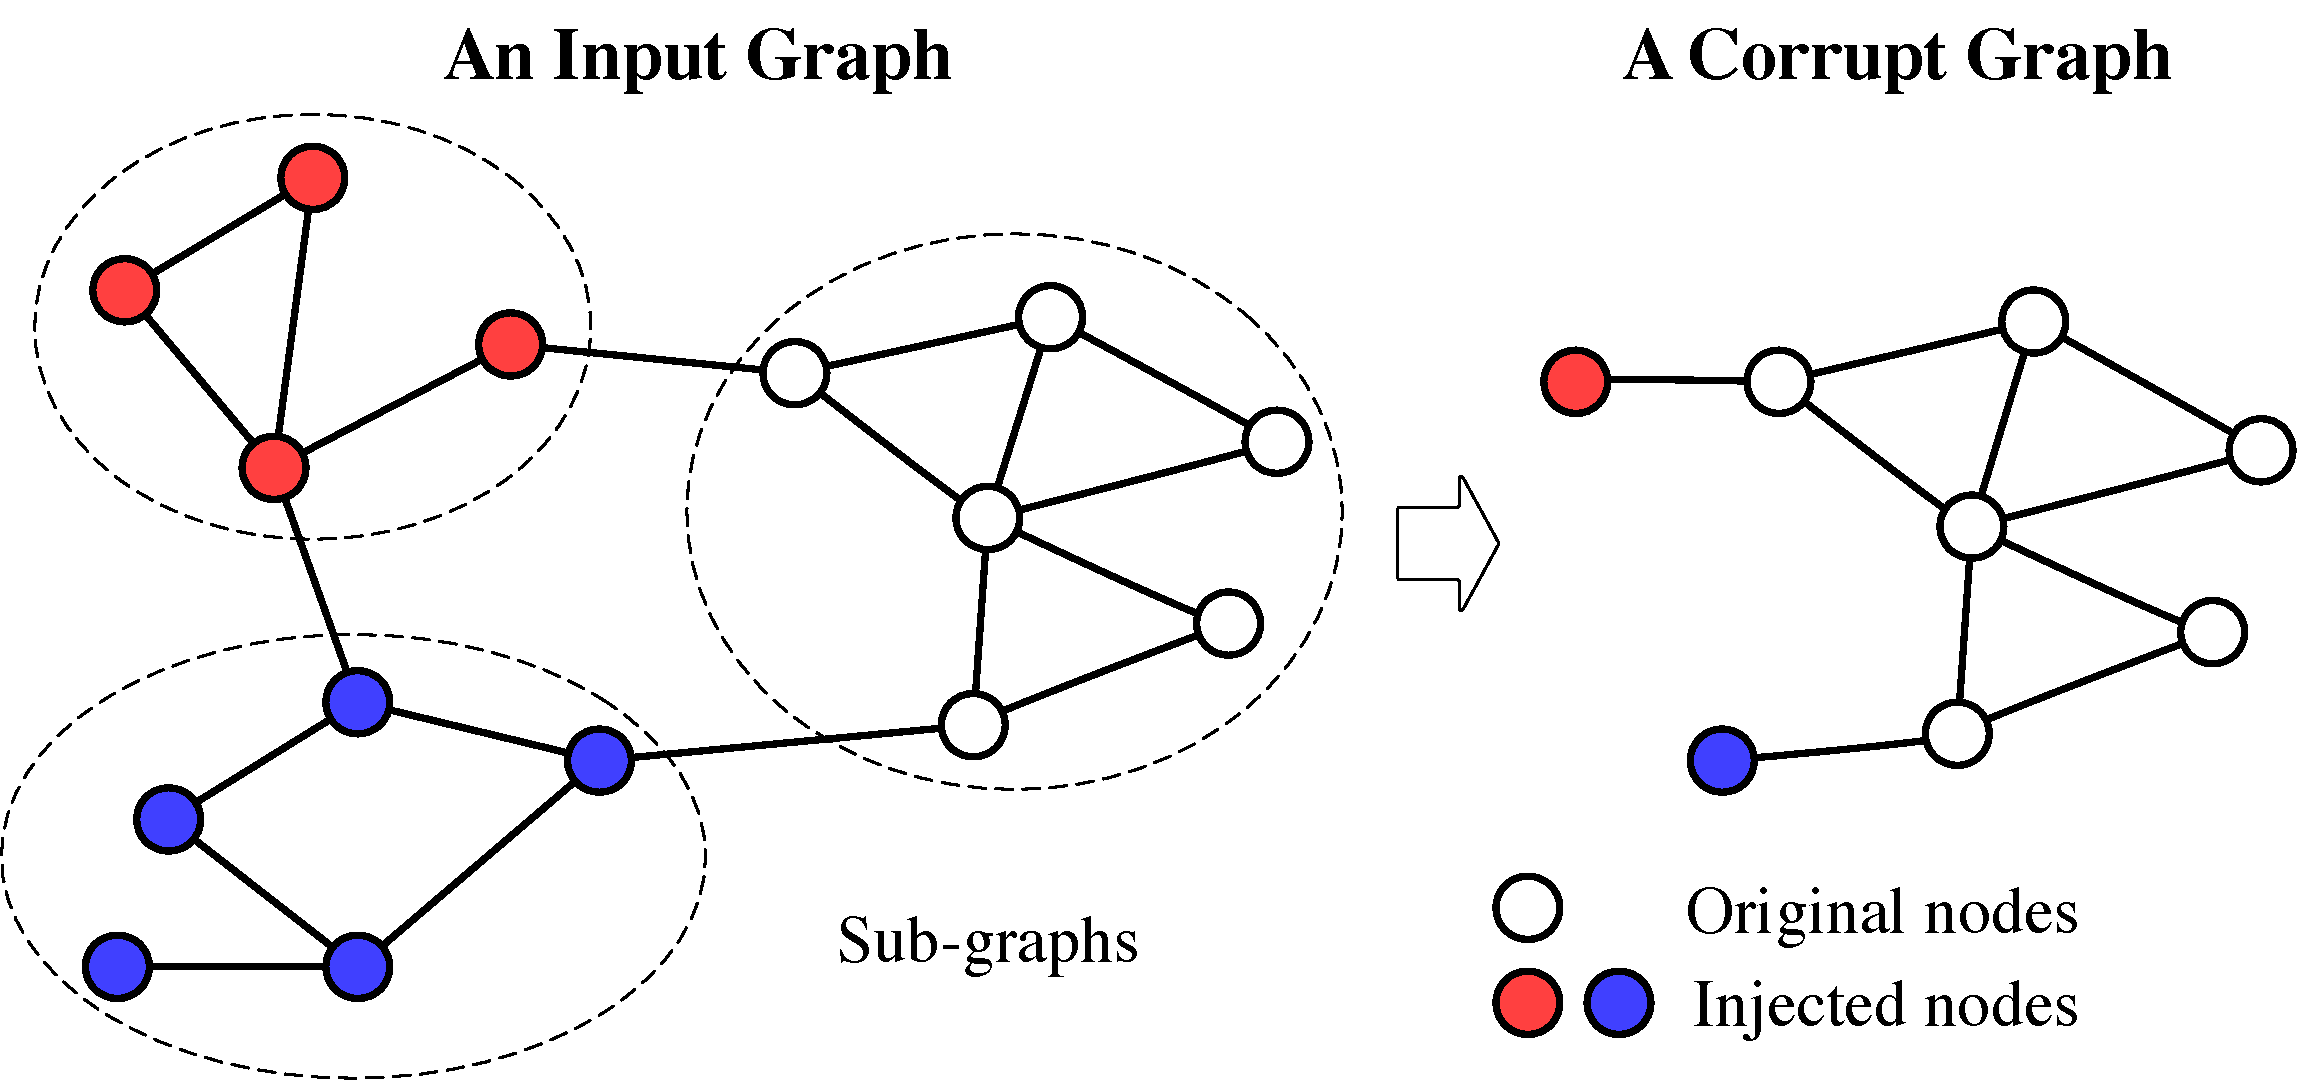
\includegraphics[width=0.4\textwidth]{figures/corrupt}
	\caption{\label{fig:corrupt} Illustration of constructing a corrupt graph. A graph is partitioned into multiple sub-graphs. A corrupt graph is constructed from each sub-graph by injecting the nodes outside it.}
\end{figure}


\vpara{Connection to Graph Pre-Training Frameworks.}
Existing graph pre-training methods offer limited benefits to anomaly detection. 
For example,  GAE~\cite{kipf2016variational} reconstruct the adjacency matrix under the local proximity assumption, which is hurt by suspicious links.
%  connecting nodes with opposite labels.
GCC~\cite{qiu2020gcc} maximizes the consistency between the sampled ego-networks of the same node compared with those sampled from different nodes, such feature consistency assumption cannot explicitly help distinguish the abnormal nodes from the normal ones. 
DGI~\cite{velickovic2019deep}, which contrasts a node with the whole graph, is akin to the contrastive objective of \pmodel, while the negative instances are addressed differently. 
In DGI, given a graph as the context, positive and negative nodes are convolved and represented in independent graphs before contrasting.
But in \pmodel, negative nodes sampled from other graphs are injected and may link to normal nodes in the corrupted graph, which increases the difficulty to distinguish normal and abnormal nodes during training, and thus improves the discrimination ability of the model. 
Essentially, DGI focuses more on representing the normal pattern while \spmodel additionally reinforces the differences of the anomalies from the normal pattern.
%Under the circumstance, benign nodes are those from original graph, yet anomaly nodes are the ones from other different graphs. Hence we can also following the optimization methods motivated by the task of instance discrimination~\cite{wu2018unsupervised} that contrasts the benign nodes and the anomaly nodes from the graph context in an unsupervised contrastive learning manner. The infoNCE loss function~\cite{oord2018representation} is the same as the one defined in section.x.










\begin{figure*}[t]
	\centering
	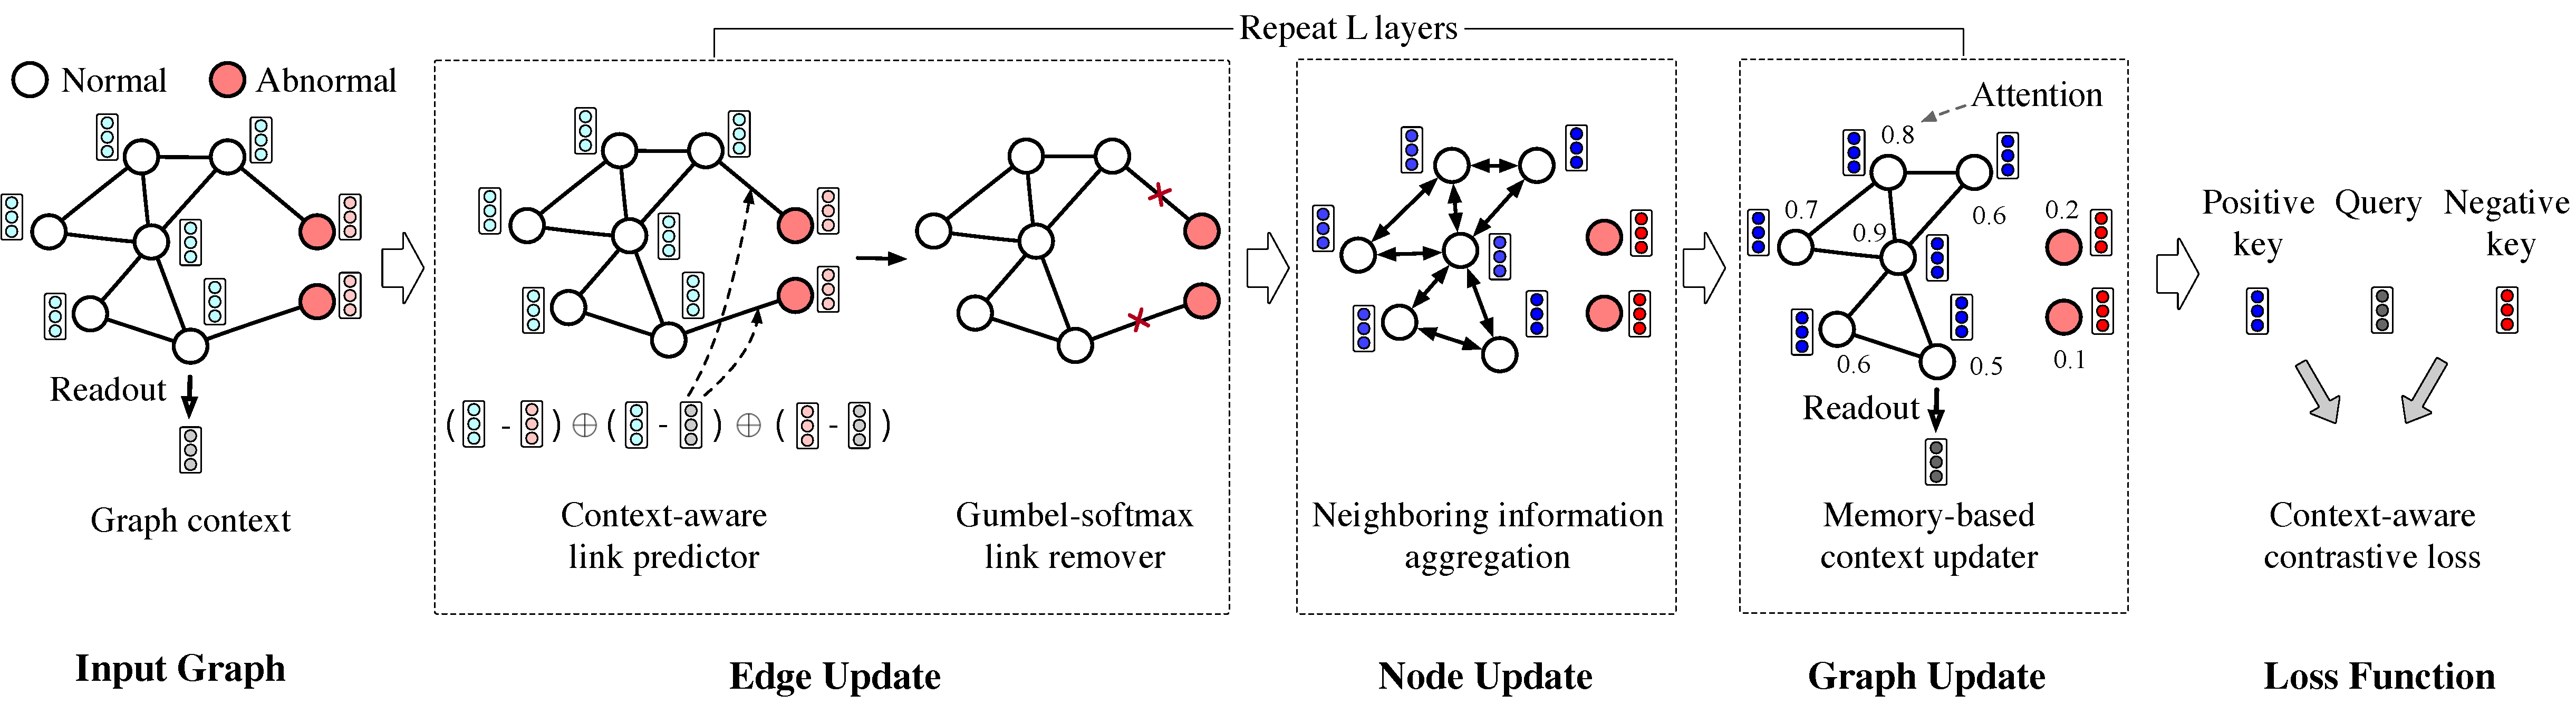
\includegraphics[width=0.9\textwidth]{figures/framework}
	\caption{\label{fig:metric_function} The framework of \model. 
		At each layer, \smodel estimates the likelihood for each edge being suspicious and then removes the most suspicious ones with the adjacency matrix updated. 
		Its next step is to update the node embeddings by message passing based on the updated adjacency matrix. 
		Finally it updates the global context. 
		After $L$-layer graph convolutions, the context-aware contrastive loss function is optimized. }
\end{figure*}



\subsection{The GNN Encoder of \model}
\label{subsec:gnn}

\subsubsection{Overview}

\hide{
To optimize the context-aware contrastive objective in Eq. \eqref{eq:loss}, in addition to the message passing and neighbor aggregation process in the general GNN models, we design 
1) an edge update step to remove the suspicious links. and
2) a graph update step to represent the global context 
That is,  \model's GNN encoder $f_{\text{GNN}}$ contains three modules: 
\begin{itemize}[leftmargin=*]
	\item \textbf{Edge Update} is to estimate the suspicious probability of a link, based on which it refines the adjacent matrix at the beginning of each convolution layer, i.e., 
	\beq{
		\label{eq:edge_update}
		{A}^{(l)} =f_{\text{edge}}\left({H}^{(l-1)}, {A}^{(l-1)}, \boldsymbol{q}^{(l-1)}\right).
	}
	\item \textbf{Node Update} is to aggregate the neighboring information based on the refined adjacent matrix ${A}^{(l)}$ and combine the aggregated result with the concerned node, i.e.,
	\beq{
		\label{eq:node_update}
		H^{(l)} = f_{\text{node}}\left(H^{(l-1)}, A^{(l)}\right).
	}
	\item \textbf{Graph Update} is to update the context of the whole graph based on the updated node embeddings $H^{(l)}$ and last-layer's graph embedding $\boldsymbol{q}^{(l-1)}$ via a readout function:  
	
	\beq{
		\label{eq:graph_udpate}
		\boldsymbol{q}^{(l)} = f_{\text{graph}}({H}^{(l)}, \boldsymbol{q}^{(l-1)}). 
	}
\end{itemize}
}

To optimize the context-aware contrastive objective in Eq. \eqref{eq:loss}, we design the edge update, node update, and graph update modules in the GNN encoder of \model. 
First, Edge update is to estimate the likelihood of each link being a suspicious one and then remove the suspicious ones. % via \textit{edge update}; 
Then, node update is to update node embeddings by message passing on the updated adjacency matrix. 
Finally, the global context is updated via graph update. 
The three modules are executed at each graph convolution layer successively. After $L$-layer forwards, the context-aware contrastive objective is optimized. 
The framework is illustrated in Fig. \ref{fig:metric_function}. 




%All existing GCN-based methods are aim at decreasing the rotten influences from anomalies with their corresponding implementing inductive bias~\cite{battaglia2018relational}. However they either suffer from limited capabilities or too rigid to generalize in different circumstances.

%In summary, we first create a new adjacency matrix $\boldsymbol{{A}}^{(l)}$ via a link predictor $f_{\text{link}}$, which estimates the suspicious likelihood of links based on the node embeddings $H^{(l-1)}$, the adjacency matrix ${A}^{(l-1)}$, and the graph context embedding $\textbf{q}^{(l-1)}$ of the last layer. Then, the node update function $f_{\text{node}}$ can be adopted to aggregate the neighboring information $H^{l-1}$ based on the adjacency matrix ${A}^{(l)}$. Finally, a readout function $f_{\text{graph}}$ is to update the graph embedding $\boldsymbol{q}^{(l)}$ via comparing the graph context $\boldsymbol{q}^{(l-1)}$ of the last layer with the updated node embeddings $H^{(l)}$. We explain the concrete design of each step as below.




\subsubsection{Edge Update} 
\hide{
We define suspicious links as the ones that connect nodes with opposite labels. 
%For example, although a paper doesn't belong to the a researcher, it may still be linked to the right papers by the same coauthor names. 
%Similarly, almost every fraudster in business websites can be linked to some benign users by the commonly rated products. 
%For example, almost every fraudster in business websites can be linked to some benign users by the commonly rated products. 
Such suspicious links violate the homophily assumption between neighbors---two neighboring nodes tend to have similar features and same labels---and impact the performance of the traditional message-passing along with the links.
}
\label{subsec:edge}
We define suspicious links as the ones that connect nodes with opposite labels. For example, almost every fraudster in business websites can be linked to some benign users by the commonly rated products. Such suspicious links violate the homophily assumption between neighbors—two neighboring nodes tend to have similar features and same labels—and impact the performance of the traditional message-passing along with the suspicious links.

Although many attempts have been made to detect such suspicious links~\cite{zhang2019key, dou2020enhancing}, 
%by attention mechanisms~\cite{wang2019semi, zhang2019key} or reinforcement learning~\cite{dou2020enhancing}, 
they merely predict the likelihood based on the linked node features regardless of the node labels. 
%In another word, they predict a high linkage likelihood for two nodes if their features are similar to each other.
%However, the links between the nodes with same labels but dissimilar features are regular and should be kept. 
Differently, we additionally model the relative distance between nodes and the global context $\boldsymbol{h}-\boldsymbol{q}$. 
The promise here is the distance can serve as implicit labels to guide the model to remove suspicious links --- those connected by the nodes with distinguished distance to the global context.
%For example, two papers of a scholar may have different topics but be linked for a few shared coauthors. 
%Reversely, two users with different preferences may also be linked as they occasionally rated the same product. 
%These links can facilitate the graph convolution of the normal nodes, smoothing their features, and benefiting the encoding of the global context. 
%\yx{to ask jing}

%Such regular links will be removed if predicting links only depending on the node features regardless of the node labels.
%Although the ground-truth labels cannot be used as features in order to avoid information leakage, we can adopt the relative distance to the global context to imply the nodes labels. 

%\yx{what is context aware in one or two sentences?}
\hide{
Thus, we propose 1) a context-aware link predictor to estimate the suspicious linkage likelihood between two nodes 
and 
2) adopt a binary Gumbel-softmax reparameterization trick~\cite{maddison2016concrete, jang2016categorical} to remove the suspicious links. 
3) perform a edge residual to smooth evolution of the edge updating.
}
\vpara{Context-Aware Link Predictor.}
The link predictor accepts the representations of two linked nodes $\boldsymbol{h}_i^{(l-1)}$ and $\boldsymbol{h}_j^{(l-1)}$ as the input, and then estimates the linkage likelihood between node $v_i$ and $v_j$ by:

\beqn{
	\label{eq:linkage_likelihood}
	p_{ij}^{(l)} = \text{MLP}\left((\boldsymbol{h}_i^{(l-1)} - \boldsymbol{h}_j^{(l-1)}) \oplus (\boldsymbol{h}_i^{(l-1)} - \boldsymbol{q}^{(l-1)})\right. \\
	\left.\oplus (\boldsymbol{h}_j^{(l-1)} - \boldsymbol{q}^{(l-1)})\right) , \nonumber
}

\noindent where $\oplus$ is the concatenation operator and MLP is a projection layer with a sigmoid activation function to normalize the likelihood into [0,1]. 
$(\boldsymbol{h}_i^{(l-1)} - \boldsymbol{h}_j^{(l-1)})$ explicitly denotes the similarity of two nodes,
while $(\boldsymbol{h}_{i}^{(l-1)} - \boldsymbol{q}^{(l-1)})$, the distance from $v_{i}$ to the global context, implicitly indicates that two nodes---even if their local features are slightly different---can be highly probably linked  given their relative positions to the global context are similar. The ablation studies in Section 3.2 empirically prove the effectiveness of this context-aware link predictor.

To accelerate the optimization of the link predictor, we optimize the prediction loss in addition to the contrastive objective in Eq.~\eqref{eq:loss}. Specifically, we treat links between normal nodes as positive ones and suspicious links as negative ones. The prediction loss is defined as

\beq{
\label{eq:constraint}
\mathcal{L}_{\text{link}} = \mathop{\mathbb{E}}\left[\sum_{i,j: y_i = y_j = 0} \!\!\!\!\!-\log p_{ij}^{(l)} - \!\!\! \sum_{\substack{i,j: y_i \neq y_j = 0} } \!\!\!\!\!\left(1-\log p_{ij}^{(l)}\right)\right],
}

\noindent which acts as the constraint to directly maximize probabilities of normal links and minimize these of suspicious ones.  



\vpara{Gumbel-softmax Link Remover.}
%The linkage likelihood $p_{ij}^{(l)}$ can be injected by attention mechanisms to distinguish the weights of different neighbors in the node update step (Eq.\eqref{eq:node_update})~\cite{wang2019semi, zhang2019key}. However, the suspicious links are not thoroughly removed and the negative influence is still propagated during message passing. Some other researchers attempt to remove the suspicious links before graph convolution~\cite{franceschi2019learning, liu2020alleviating}. Since the link removing and the graph convolution are decoupled, the gradient cannot be passed to the link predictor during backward procedure. 
We remove the suspicious links to reduce their negative influence thoroughly by employing the Bernoulli approximation, the binary case of the Gumbel-softmax reparameterization trick~\cite{maddison2016concrete, jang2016categorical} to resolve the discrete non-differentiable problem.
%deal with the gradient vanishing issue caused by discrete sampling actions. 
Specifically, we define the indicator matrix $I \in \mathbb{R}^{N \times N}$, and for the link likelihood $p_{ij}^{(l)}$, 
we decide whether to keep the link $(I^{(l)}_{ij} = 1)$ or not $(I^{(l)}_{ij}=0)$ by the following equation: 

% \beq{
% 	\label{eq:GUMBEL}
% 	I^{(l)}_{ij} = \left \lfloor \frac{1}{1 + \exp \left(-(\log p_{ij}^{(l)}+ \varepsilon)/\lambda \right)} + \frac{1}{2} \right \rfloor,
% }


\beq{
	\label{eq:GUMBEL}
	I^{(l)}_{ij} = \text{Bernoulli}\left[\frac{1}{1 + \exp \left(-(\log p_{ij}^{(l)}+ \varepsilon)/\lambda \right)}\right],
}


\noindent where $\text{Bernoulli (p)}$ is the Bernoulli approximation with the probability $\text{p}$ to keep the link, $\lambda$ is the temperature hyper-parameter to control the sharpness of the sampling process (the lower $\lambda$ is, the more links will be kept), 
and $\varepsilon \sim \text{Gumbel}~(0,1)$ is the Gumbel noise for reparameterization.
In the forward process, we sample according to Eq.~\eqref{eq:GUMBEL} to obtain $I^{(l)}_{ij}$. 
In the backward process, a straight-through gradient estimator~\cite{bengio2013estimating} is employed to pass the gradients to the relaxed value $p_{ij}^{(l)}$ instead of the discrete value ${I}^{(l)}_{ij}$. %Practically, we adopt the tools provided by pyro, a universal probabilistic programming language\footnote{https://pyro.ai/}. 

 %To enable the discrete sampling of the links, we further 
%Then we adopt  the straight-through gradient estimator~\cite{bengio2013estimating} to round $\tilde{p}^{(l)}_{ij}$ as 1 if it is larger than 0.5 and 0 otherwise and assign the discrete value to ${A}_{ij}^{(l)}$ for the forward computation, 
%According to straight-through gradient estimator~\cite{bengio2013estimating}, we pass the gradients to the relaxed value $p_{ij}^{(l)}$  instead of the discrete value ${A}^{(l)}_{ij}$ during the backward procedure. 

\vpara{Edge Residual.} Recently, RealFormer~\cite{he2020realformer} verifies the effect of the residual connection of attention scores. Inspired by this, we perform the residual connection of the original edge likelihood and the estimated edge likelihood to smooth the edge evolution as follows:

\beq{
A_{ij}^{(l)} = \left(\alpha A_{ij}^{(l-1)} + (1-\alpha) p_{ij}^{(l)}\right) \odot I^{(l)}_{ij},
}

\noindent where $\alpha$ is a learnable parameter to balance the weight from the last layer and the estimated weight $p_{ij}$, and $\odot$ denotes the Hadamard product. 
%which rounds the relaxed samples in Eq.\eqref{eq:GUMBEL} during the forward procedure, 


\hide{
\beqn{
	\label{eq:round}
	{A}^{(l)}_{ij}  &=& \left\{\begin{array}{cl} 
		1 & \tilde{p}^{(l)}_{ij} \geq 0.5;   \\ 
		0 & \mbox{otherwise,}   
	\end{array}\right.  \\  \nonumber
}
}

%\noindent but passes the gradients to the relaxed samples in Eq.\eqref{eq:GUMBEL} rather than the rounded values in  Eq.\eqref{eq:round} during the backward procedure.




\subsubsection{Node Update}
Updating node embeddings can be divided into an AGGREGATION and a COMBINE operation:

\beqn{
	\label{eq:aggregation}
	\boldsymbol{a}_i^{(l)}\!\!\! &=& \!\!\!\text{AGGREGATION}(\{\boldsymbol{h}_{j}^{(l-1)}: A_{ij}^{(l)} > 0\}), \\
	\label{eq:combination}
	\boldsymbol{h}_{i}^{(l)} \!\!\!&=&\!\!\! \text{COMBINE}(\boldsymbol{h}_i^{(l-1)}, \boldsymbol{a}_i^{(l)}),
}

\noindent where Eq. \eqref{eq:aggregation} is to aggregate the neighboring messages of the last layer based on the updated adjacency matrix and Eq.\eqref{eq:combination} is to combine the aggregated information with the concerned node. Generally, the two operations are flexible enough to fit any GNNs. Experiments in \secref{sec:exp} have investigated several concrete functions.

%The AGGREGATION operation is the sum, the same as GIN~\cite{xu2018powerful}, and the COMBINE operation is concatenation. 


\subsubsection{Graph Update}
%The graph embedding $\boldsymbol{q}$, i.e., the global context, needs to be updated at each layer after all nodes' embeddings are updated. 
Straightforwardly, we can perform sum, max, or average pooling of all the nodes to update the global context. However, they do not distinguish the normal and abnormal nodes, which results in an inaccurate global context. To alleviate it, we introduce a memory buffer $\boldsymbol{m}$ to register the global context $\boldsymbol{q}^{(l-1)}$ of the last layer, based on which we calculate the contribution of each node to the global context. The assumption is a node that is deviated from the current global context should be weakened in the next update step. Such the memory-based mechanism has been successfully applied to general computation machines~\cite{bahdanau2015neural, weston2014memory}. Formally,

\beqn{
	\label{eq:readout}
	&&\!\!\!\!\!\!\!\!\!\!\!\!\!\! s_i^{(l)} = \text{cosine}\left( \boldsymbol{h}_i^{(l)}, \boldsymbol{m}\right), \quad \alpha_i^{(l)} = \frac{\exp (s_i^{(l)})}{\sum_{j=1}^{N}\exp(s_j^{(l)})}, \\ \nonumber
	&& \!\!\!\!\!\! \boldsymbol{q}^{(l)} = \sum_{i=1}^{N}\alpha_i^{(l)} \cdot \boldsymbol{h}_i^{(l)}, \quad \boldsymbol{m} = \boldsymbol{q}^{(l)}.
}

First, we compute the attention $\alpha_i^{(l)}$ for each node $v_i$ based on its cosine similarity with the memory vector. Then we update the global context $\boldsymbol{q}^{(l)}$ by weighted aggregating different nodes and update the memory vector $\boldsymbol{m}$. 
Such a memory-based graph update strategy can get rid of the negative influence of the abnormal nodes on the ``positive" global context as much as possible.

%===============================================================
	\begin{algorithm}[t]
		\label{al: algo}
		{\small \caption{\smodel or \pmodel\label{algo:training}}
			\KwIn{A set of labeled/pseudo-labeled graphs $\{G_i\}_{i=1}^M$. Each graph $G_i$ is consist of the adjacency matrix $A \in \mathbb{R}^{N \times N}$, and feature matrix ${X} \in \mathbb{R}^{N \times d}$. Also the learning rate $\eta$, an $L$-layers GNNs encoder: $f_{\text{GNN}}({X}, {A}, {W})$.} 
			\KwOut{Learned parameter $W$ of $f_{\text{GNN}}$, where $W = \{W_{\text{edge}}, W_{\text{node}}, W_{\text{global}}\}$}
			Initialize the global context $\boldsymbol{q}^{(0)} = \frac{1}{N}(\sum_{j=1}^{N}\boldsymbol{x}_j)$; \\
			Initialize the trainable parameter $W$ of $f_{\text{GNN}}$; \\			
			\Repeat{Converges}{
				\ForEach{ $G_i$}{
					\For{ $l$ from 1 to $L$}{
						Edge update to get the adjacency matrix: 
						${A}^{(l)}=f_{\text{edge}}\left({H}^{(l-1)}, {A}^{(l-1)}, \boldsymbol{q}^{(l-1)}, W_{\text{edge}}\right)$.\\
						Node update to get the node embeddings:
						$H^{(l)} = f_{\text{node}}\left(H^{(l-1)}, A^{(l)}, W_{\text{node}}\right)$.\\
						Graph update to get the global context:
						$\boldsymbol{q}^{(l)} = f_{\text{graph}}({H}^{(l)}, \boldsymbol{q}^{(l-1)}, W_{\text{global}})$\\
					}
					Compute the loss function in Eq.~\eqref{eq:final}.\\
					Update $W$ by $W = W - \eta \nabla_{W} \mathcal{L}$;\\
				}
			}
		}
	\end{algorithm}
%===============================================================




\subsection{Training and Inference}
% Instead of directly predicting a binary label for each node, for node $v_i \in G$ to be predicted, we get its embedding $\boldsymbol{h}_i^{(L)}$ and the graph embedding $\boldsymbol{q}^{(L)}$ of the final layer, and compute the cosine similarity between them as the abnormal extent of $v_i$ (the lower, the more anomalous).

In each epoch, we optimize both the context-aware contrastive loss in Eq.~\eqref{eq:loss} and the link predictor constraint loss in Eq.~\eqref{eq:constraint} as follows:

\beq{
\label{eq:final}
\mathcal{L} = \mathcal{L}_{\text{con}} + \lambda \mathcal{L}_{\text{link}},
}

\noindent where $\lambda$ is a balanced hyper-parameter. We empirically set $\lambda$ as 0.2 in our model. Algorithm~\ref{al: algo} outlines the training process. 
During inference, for node $v_i$ to be predicted, instead of directly predicting a binary label, we estimate its abnormality score by computing the cosine similarity between its embedding $\boldsymbol{h}_i^{(L)}$ and the graph embedding $\boldsymbol{q}^{(L)}$ of the final layer (the lower, the more anomalous).

\subsection{Complexity}
The time complexity of \smodel is the same order of magnitude as the vanilla GNN.
Because on top of the node update step of GNN, \smodel adds two additional efficient steps, edge update, and graph update. The time complexity of edge update in layer $k$ is $\mathcal{O}\left(D_kE\right)$, where $E$ is the number of edges and $D_k$ is the embedding size in layer $k$. 
The time complexity of graph update in layer $k$ is $\mathcal{O}\left(D_kN\right)$, where $N$ is the number of nodes. Since the embedding size is far smaller than the number of nodes or edges, the time complexity of \smodel grows linearly with the graph scale, which is the same as the vanilla GNN.





























\hide{



\section{Graph-based Anomaly Detection}
\label{sec:approach}


In this section, we formalize the problem of graph-based anomaly detection. To address it, we present the context-aware graph contrastive learning (\model) model and further extent it to \spmodel in an unsupervised manner.

\subsection{Graph-based Anomaly Detection Problem}
We denote a graph as $G = \left(V, X, A\right)$, where $V$ is the set of $N$ nodes and ${X}$ is the corresponding feature vectors, with $\boldsymbol{x}_i \in \mathbb{R}^d$ denoting the $d$-dimensional feature vector of $v_i$. Notation $A \in \mathbb{R}^{N \times N}$ represents the adjacency matrix. 
Generally, $A$ can carry arbitrary edge features to represent various graph properties such as the unweighted or weighted, the undirected or directed, and the single-relational or multi-relational graphs. 
To generalize to various scenarios of anomaly detection, we simplify $G$ into an unweighted, undirected and single-relational graph. Therefore, $A_{ij} = 1$ if there exists an edge between $v_i$ and $v_j$ in ${G}$ and $A_{ij} = 0$ otherwise.

\begin{problem}
	
	\textbf{Anomaly Detection on Graphs.} 
	Given a labeled graph $G = \left(V, X, A, Y\right)$, $Y$ is the set of labels on nodes and each $y_i \in Y$ is a binary value which takes value 1 if the corresponding node $v_i$ is abnormal and 0 otherwise. We need to learn a predictive function $f: V \rightarrow \mathbb{R}^d$ that maps nodes to a $d$-dimensional space, where $d \ll |V|$. The function $f$ needs to preserve both the structural information and the input features of the nodes. With the learned node embeddigns, we aim to learn a classifier $g: \mathbb{R}^d \rightarrow \{0,1\}$ to determine whether a given node is abnormal (1) or normal (0). 
\end{problem}

\subsection{\smodel}
\subsubsection{Context-aware Contrastive Loss Function}
Existing GNN-based methods instantiate $f$ as a GNN encoder (i.e., $f_{\text{GNN}}$) and $g$ as a discriminative layer such as MLP, to directly map a node embedding into a binary value~\cite{dou2020enhancing,liu2020alleviating}. 
However, anomaly detection cannot be simply treated as a general binary classification problem, because the abnormal nodes as well as the normal nodes present diverse feature distributions, which makes it challenging to find a clear boundary by binary classification. 
For example, in Figure 1, for cleaning the researcher's profiles, the wrong papers denoted by red nodes distinguish from the normal pattern in various aspects, i.e., the features of wrong papers are not consistent. 
Similarly, for detecting the fraudsters who publish malicious comments on products in business websites, the fraudsters may comment on different kinds of products. 
Simultaneously, the normal nodes may also present diverse patterns due to diverse preferences. 
%For example,  a researcher may publish papers in multiple topics with different groups of coauthors in various venues, resulting in a diverse paper network. Similarly, the abnormal users in business websites may favour different categories of products. 
Such diverse features of the abnormal and the normal nodes will hurt the performance of node binary classification.

Despite the irregular node features, we discover the difference of the distance to the global context between the normal nodes and the abnormal nodes; that is, the anomalous extent of a node depends more on its deviation from the majority of the nodes than its own features.
In view of this, we propose a context-aware graph contrastive objective function instead of the binary classification objective function. The basic idea is to determine a node's label via contrasting it with the global context of the entire graph. %The underlying assumption is a node is more abnormal if it deviates farther away from the whole context. 
Specifically, given a graph ${G}$, we first create a GNN encoder $f_{\text{GNN}}$ that can output an embedding $\boldsymbol{h}_i$ for each node $v_i$ and also an embedding $\boldsymbol{q}$ for the entire graph (global context), i.e., ${H}, \boldsymbol{q} = f_{\text{GNN}}({X}, {A})$ with $H = \{\boldsymbol{h}_i\}_{i=1}^{N}$. We take the graph embedding as the query, a normal node's embedding as the positive key that matches with $\boldsymbol{q}$ together with the embeddings of the all the abnormal nodes as the negative keys that don't match with $\boldsymbol{q}$. 
For implementation, we use infoNCE~\cite{oord2018representation}, the well-adopted loss function in contrastive learning, as the concrete loss function such that:


\beq{
	\label{eq:loss}
	\mathcal{L} = \sum_{i: y_i = 0 } \left[-\log \frac{\exp \left(\textbf{q}^\top\boldsymbol{h}_i/\tau\right)}{ \sum_{ j: y_j = 1} \exp \left(\boldsymbol{q}^\top \boldsymbol{h}_j/\tau\right) + \exp \left(\boldsymbol{q}^\top\boldsymbol{h}_i/\tau\right) }\right],
}

\noindent where $\tau$ is the temperature hyperparameter. The objective function is to enforce maximizing the consistency between the positive pairs (normal node, global context) compared with negative pairs (abnormal node, global context). 

\vpara{Connections with Other Graph Contrastive Learning Frameworks.}
\smodel is different from the existing graph contrastive learning frameworks for GNN pre-training, because most of them are unsupervised and the contrastive instances should be constructed from the unlabeled data.  
For example, in GCC~\cite{qiu2020gcc}, given the embedding of a randomly sampled ego-network of a node as the query, the positive key is the embedding of another sampled ego-network of the same node, and the negative keys are those sampled from other nodes. 
In DGI~\cite{velickovic2019deep} and GraphCL~\cite{you2020graph}, given the entire graph embedding as the query, the positive key is the embedding of a node in it, and the negative keys are the embeddings of the same node after permutating the graph. In contrast, in our objective function for anomaly detection, the positive and the negative keys are constrained to the normal and abnormal nodes respectively, which can be treated as supervised contrastive learning~\cite{khosla2020supervised}. But different from supervised contrastive learning that discriminates between the features of instances, 
we inject global context and compare the relative distance to this context between instances to overcome the feature diversity issue. 
\smodel  combines the advantages of the existing frameworks and can be viewed a supervised context-aware contrastive learning framework.



\begin{figure*}[t]
	\centering
	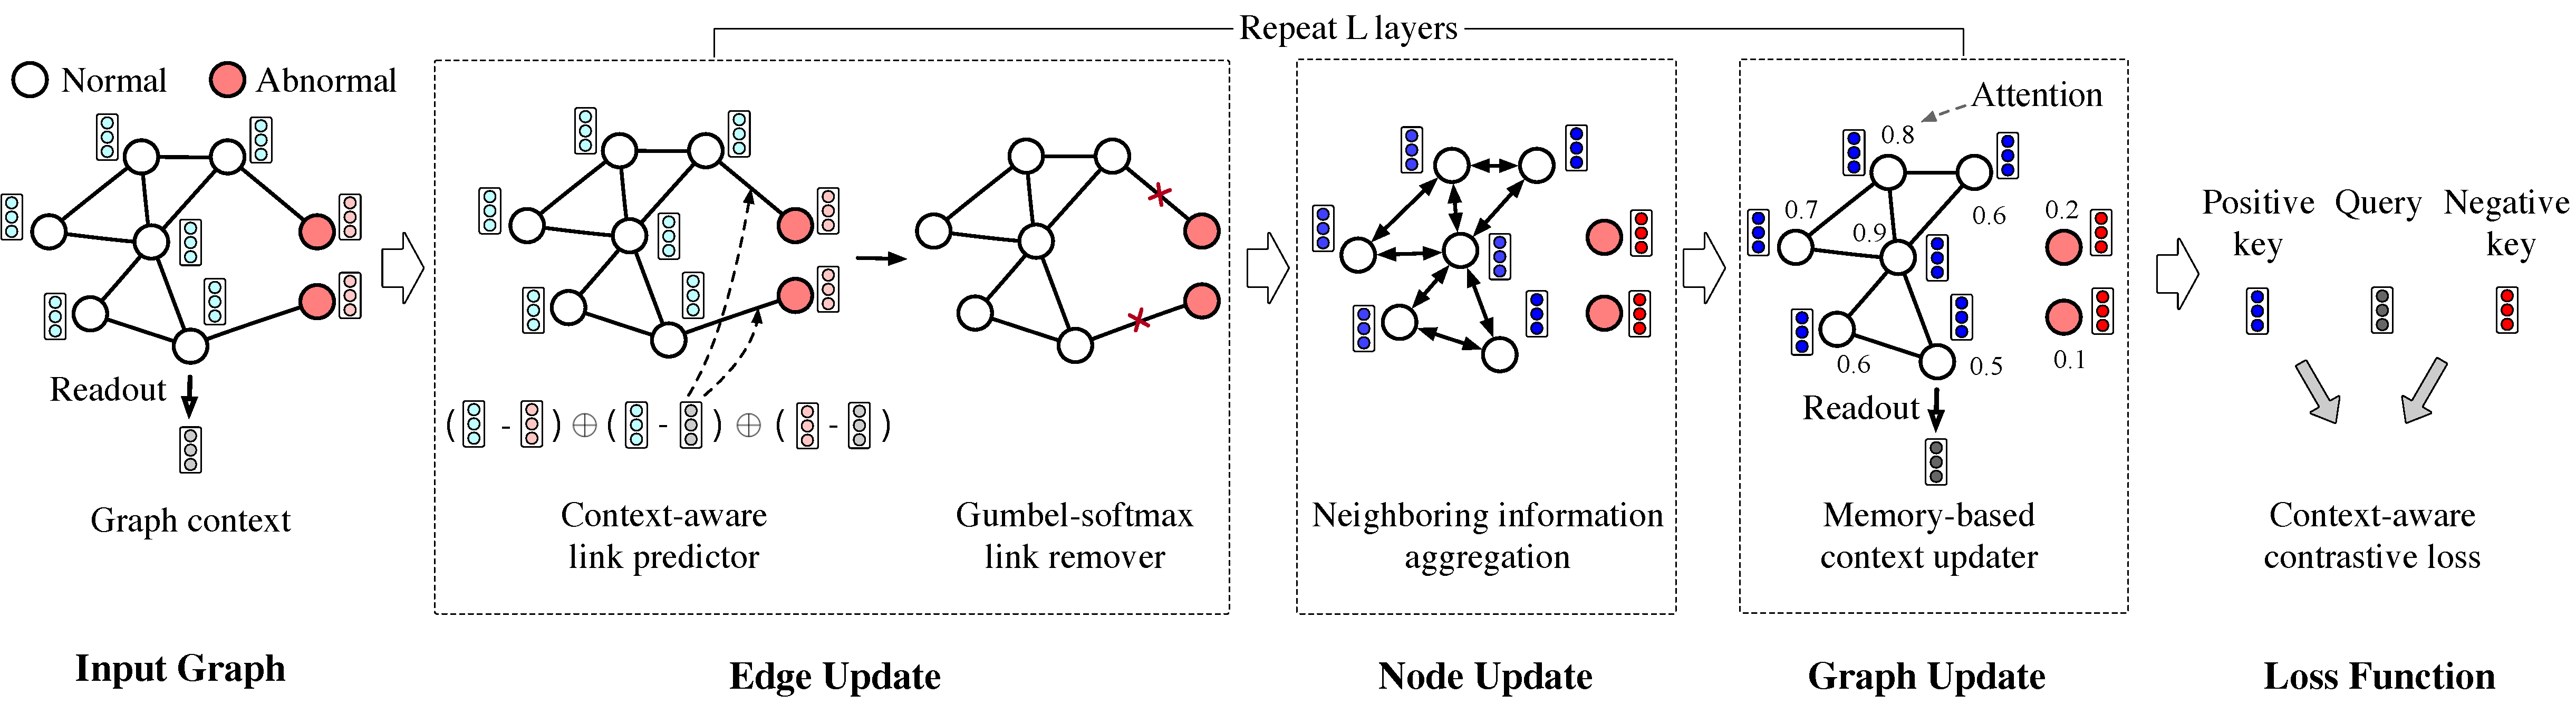
\includegraphics[width=\textwidth]{figures/framework}
	\caption{\label{fig:metric_function} The framework of \model. At each layer, \smodel estimates the linkage likelihood for each link and remove the most suspicious ones. Then based on the udpated adjacency matrix, it updates the node embeddings by message passing and finally updates the global context. After $L$-layer graph convolutions, the context-aware contrastive loss function is optimized. }
\end{figure*}


\subsubsection{GNN Encoder $f_{\text{GNN}}$ }
%All existing GCN-based methods are aim at decreasing the rotten influences from anomalies with their corresponding implementing inductive bias~\cite{battaglia2018relational}. However they either suffer from limited capabilities or too rigid to generalize in different circumstances.

To achieve the context-aware contrastive objective, in addition to the message passing and neighbor aggregation process in the general GNN models, we add a graph update step to represent the global context as well as an edge update step to remove the suspicious links.
Thus $f_{\text{GNN}}$ contains three steps:

\begin{itemize}[leftmargin=*]
	\item \textbf{Edge Update} is to estimate the suspicious probability of a link and modify the adjacent matrix according to the probabilities at the beginning of each convolution layer, i.e., 
	
	\beq{
		\label{eq:edge_update}
		{A}^{(l)} =f_{\text{link}}\left({H}^{(l-1)}, {A}^{(l-1)}, \boldsymbol{q}^{(l-1)}\right).
	}
	
	\item \textbf{Node Update} is to aggregate the neighboring information based on the modified adjacent matrix ${A}^{(l)}$ and then combine the aggregated result with the concerned node, i.e.,
	
	\beq{
		\label{eq:node_update}
		H^{(l)} = f_{\text{node}}\left(H^{(l-1)}, A^{(l)}\right).
	}
	
	\item \textbf{Graph Update} is to update the context of the whole graph based on the updated node embeddings $H^{(l)}$ and last-layer's graph embedding $\boldsymbol{q}^l$ via a readout function:  
	
	\beq{
		\label{eq:graph_udpate}
		\boldsymbol{q}^{(l)} = f_{\text{graph}}({H}^{(l)}, \boldsymbol{q}^{(l-1)}). 
	}
	
\end{itemize}

%In summary, we first create a new adjacency matrix $\boldsymbol{{A}}^{(l)}$ via a link predictor $f_{\text{link}}$, which estimates the suspicious likelihood of links based on the node embeddings $H^{(l-1)}$, the adjacency matrix ${A}^{(l-1)}$, and the graph context embedding $\textbf{q}^{(l-1)}$ of the last layer. Then, the node update function $f_{\text{node}}$ can be adopted to aggregate the neighboring information $H^{l-1}$ based on the adjacency matrix ${A}^{(l)}$. Finally, a readout function $f_{\text{graph}}$ is to update the graph embedding $\boldsymbol{q}^{(l)}$ via comparing the graph context $\boldsymbol{q}^{(l-1)}$ of the last layer with the updated node embeddings $H^{(l)}$. We explain the concrete design of each step as below.



\vpara{Edge Update.} 
The suspicious links are the links that connect nodes with opposite labels. For example, although a paper doesn't belong to the a researcher, it may still be linked to the right papers by the same coauthor names. Similarly, almost every fraudster in business websites can be linked to some benign users by the commonly rated products. Such suspicious links violate the homophily assumption between neighbors---two neighboring nodes tend to have similar features and same labels---and impact the performance of the traditional message-passing along the links.

Although existing attempts have been made to address such suspicious links by attention mechanisms~\cite{wang2019semi, zhang2019key} or reinforcement learning~\cite{dou2020enhancing}, they predict the likelihood of a link only based on the node features regardless of the node labels. 
In another word, they predict a high linkage likelihood for two nodes if their features are similar to each other.
However, the links between the nodes with same labels but dissimilar features are regular and should be kept.
For example, two papers of a researcher may have different topics but be linked for a few shared coauthors. 
Similarly, two users with different preferences may be linked as they occasionally rated the same product. 
These links can facilitate the graph convolution of the normal nodes, smoothing their features and benefiting the encoding of the global context. 
Such regular links will be removed if predicting links only depending on the node features regardless of the node labels.
Although for avoiding information leakage, the ground-true labels cannot be used as features, we can adopt the relative distance to the global context to imply the nodes labels.

Thus, we propose 1) a context-aware link predictor to estimate the linkage likelihood between two nodes and 2) adopt a binary Gumbel-softmax reparameterization trick~\cite{maddison2016concrete, jang2016categorical} to remove the suspicious links.

\ipara{Context-aware Link Predictor.}
The link predictor accepts the representations of two nodes as the input, where each node is represented by its own embedding and its relative distance to the global context embedding, i.e.,

\beq{
	\label{eq:node_feature}
	\tilde{\boldsymbol{h}}_i^{(l-1)} = \text{MLP}\left(\boldsymbol{h}_i^{(l-1)} \oplus (\boldsymbol{h}_i^{(l-1)} - \boldsymbol{q}^{(l-1)})\right),
} 

\noindent where $\oplus$ is the concatenation operator and MLP is a projection layer. $(\boldsymbol{h}_i^{(l-1)} - \boldsymbol{q}^{(l-1)})$, the distance from $v_i$ to the global context, indicates that two nodes---even if their local features are slightly different---can be highly probably linked  provided their relative positions to the global context are similar. 
Then, the linkage likelihood between node $v_i$ and $v_j$ can be calculated as 

\beq{
	\label{eq:linkage_likelihood}
	p_{ij}^{(l)} = \text{ReLU} \left( \text{cosine} (\tilde{\boldsymbol{h}}^{(l-1)}_i, \tilde{\boldsymbol{h}}^{(l-1)}_j)\right),
}

\noindent where $\text{ReLU}$ normalizes the cosine similarities into [0,1].

\ipara{Gumbel-Softmax Link Remover.}
%The linkage likelihood $p_{ij}^{(l)}$ can be injected by attention mechanisms to distinguish the weights of different neighbors in the node update step (Eq.\eqref{eq:node_update})~\cite{wang2019semi, zhang2019key}. However, the suspicious links are not thoroughly removed and the negative influence is still propagated during message passing. Some other researchers attempt to remove the suspicious links before graph convolution~\cite{franceschi2019learning, liu2020alleviating}. Since the link removing and the graph convolution are decoupled, the gradient cannot be passed to the link predictor during backward procedure. 
We remove the suspicious links to reduce the negative influence from them thoroughly by employing Bernoulli approximation, the binary case of the Gumbel-Softmax reparameterization trick~\cite{maddison2016concrete, jang2016categorical}.
%deal with the gradient vanishing issue caused by discrete sampling actions. 
Specifically, for each link $A_{ij}^{(l)}$, we first sample a Gumbel noise $\varepsilon \sim Gumbel~(0,1)$, add it to the logarithm of the linkage likelihood $p_{ij}^{(l)}$, and then apply a sigmoid function to get an updated score

\beq{
	\label{eq:GUMBEL}
	\tilde{p}^{(l)}_{ij} = \left \lfloor \frac{1}{1 + \exp \left(-(\log p_{ij}^{(l)}+ \varepsilon)/\lambda \right)} + \frac{1}{2} \right \rfloor,
}

\noindent which highly approximates  the binary value sampled according to $p_{ij}^{(l)}$. Notation $\lambda$ indicates the temperature of Gumbel-Softmax distribution. %To enable the discrete sampling of the links, we further 
Then we adopt  the straight-through gradient estimator~\cite{bengio2013estimating} to round $\tilde{p}^{(l)}_{ij}$ as 1 if it is larger than 0.5 and 0 otherwise and assign the discrete value to ${A}_{ij}^{(l)}$ for the forward computation, but pass the gradients to the relaxed values in Eq.\eqref{eq:GUMBEL} during the backward procedure. To accelerate the optimization of the link predictor, we also add $\mathcal{L}_{\text{link}} = \sum_{i,j: A^{(l-1)}_{ij} = 1} -\log p_{ij}^{(l)}$, the cross-entropy loss between the  estimated likelihood $p_{ij}^{(l)}$ and the observation $A^{(l-1)}_{ij}$ of the last layer, as the constraint of the contrastive loss function in Eq.\eqref{eq:loss}.


%which rounds the relaxed samples in Eq.\eqref{eq:GUMBEL} during the forward procedure, 


\hide{
\beqn{
	\label{eq:round}
	{A}^{(l)}_{ij}  &=& \left\{\begin{array}{cl} 
		1 & \tilde{p}^{(l)}_{ij} \geq 0.5;   \\ 
		0 & \mbox{otherwise,}   
	\end{array}\right.  \\  \nonumber
}
}

%\noindent but passes the gradients to the relaxed samples in Eq.\eqref{eq:GUMBEL} rather than the rounded values in  Eq.\eqref{eq:round} during the backward procedure.




\vpara{Node Update.}
For updating node embeddings, Eq.\eqref{eq:node_update} is divided into an AGGREGATION and a COMBINE operations:

\beqn{
	\label{[eq:aggregation}
	\boldsymbol{a}_i^{(l)} &=& \text{AGGREGATION}(\{\boldsymbol{h}_{j}^{(l-1)}: A_{ij}^{(l)} = 1\}), \\
	\label{eq:combination}
	\boldsymbol{h}_{i}^{(l)} &=& \text{COMBINE}(\boldsymbol{h}_i^{(l-1)}, \boldsymbol{a}_i^{(l)}),
}

\noindent where Eq.\eqref{[eq:aggregation} is to aggregate the neighboring information of the last layer based on the updated adjacency matrix and Eq.\eqref{eq:combination} is to combine the aggregated neighboring information with the concerned node. The AGGREGATION operation is max, the same as the state-of-the-art GIN, and the COMBINAE operation is concatenation. 


\vpara{Graph Update.}
The graph embedding $\boldsymbol{q}$, i.e., the global context, needs to be updated at each layer after all nodes' embeddings are updated. Straightforwardly, we can perform sum, max or average pooling of all the nodes to represent the global context. However, they do not distinguish the normal and abnormal nodes, which result in the inaccurate global context being deviated from the normal pattern. To tackle the problem, we introduce a memory buffer $\boldsymbol{m}$ to register the global context $\boldsymbol{q}^{(l-1)}$ of the last layer, based on which we calculate the contribution of each node to the global context. The assumption is a node that is deviated from current global context should be weakened in the next context update step. Such memory-based mechanism has been successfully applied to machine translation~\cite{vinyals2015order, bahdanau2015neural} and more general computation machines~\cite{weston2014memory, graves2014neural}. The concrete strategy can be formulated as follows:

\beqn{
	\label{eq:readout}
	&&s_i^{(l)} = \text{cosine}\left( \boldsymbol{h}_i^{(l)}, \boldsymbol{m}\right), \quad \alpha_i^{(l)} = \frac{\exp (s_i^{(l)})}{\sum_{j=1}^{N}\exp(s_j^{(l)})}, \\ \nonumber
	&&\boldsymbol{q}^{(l)} = \sum_{i=1}^{N}\alpha_i^{(l)} \cdot \boldsymbol{h}_i^{(l)}, \quad \boldsymbol{m} = \boldsymbol{q}^{(l)}.
}

In the above equation, we read out the memory and compute the attention $\alpha_i^{(l)}$ for each node $v_i$ based on its cosine similarity with the memory vector. Then we update the global context $\boldsymbol{q}^{(l)}$ by weightedly aggregating different nodes and write it into the memory to update the memory vector $\boldsymbol{m}$. 


\hide{
	\begin{algorithm}[t]
		{\small \caption{Training Process of \model or \pmodel\label{algo:training}}
			\KwIn{A set of labeled/pseudo-labeled graphs $\{G_i\}_{i=1}^M$.}
			\KwOut{Learned parameters in $f_{\text{GNN}}$.}
			\Repeat{Converges}{
				\ForEach{ $G_i$}{
					\For{ $l$ from 1 to $L$}{
						Perform edge-update step to get $A^{(l)}$ by Eq.\eqref{eq:edge_update};\\
						Perform node-update step to get $H^{(l)}$ by Eq.\eqref{eq:node_update};\\
						Perform graph-update step to get $\boldsymbol{q}^{(l)}$ by Eq.\eqref{eq:graph_udpate};\\
					}
					Perform gradient decent on the summed loss of Eq.\eqref{eq:loss} and Eq.\eqref{eq:link_loss};\\
				}
			}
		}
	\end{algorithm}
}


\subsection{\spmodel for Unsupervised Setting}
\label{sec:corrupt_graph}
\begin{figure}[t]
	\centering
	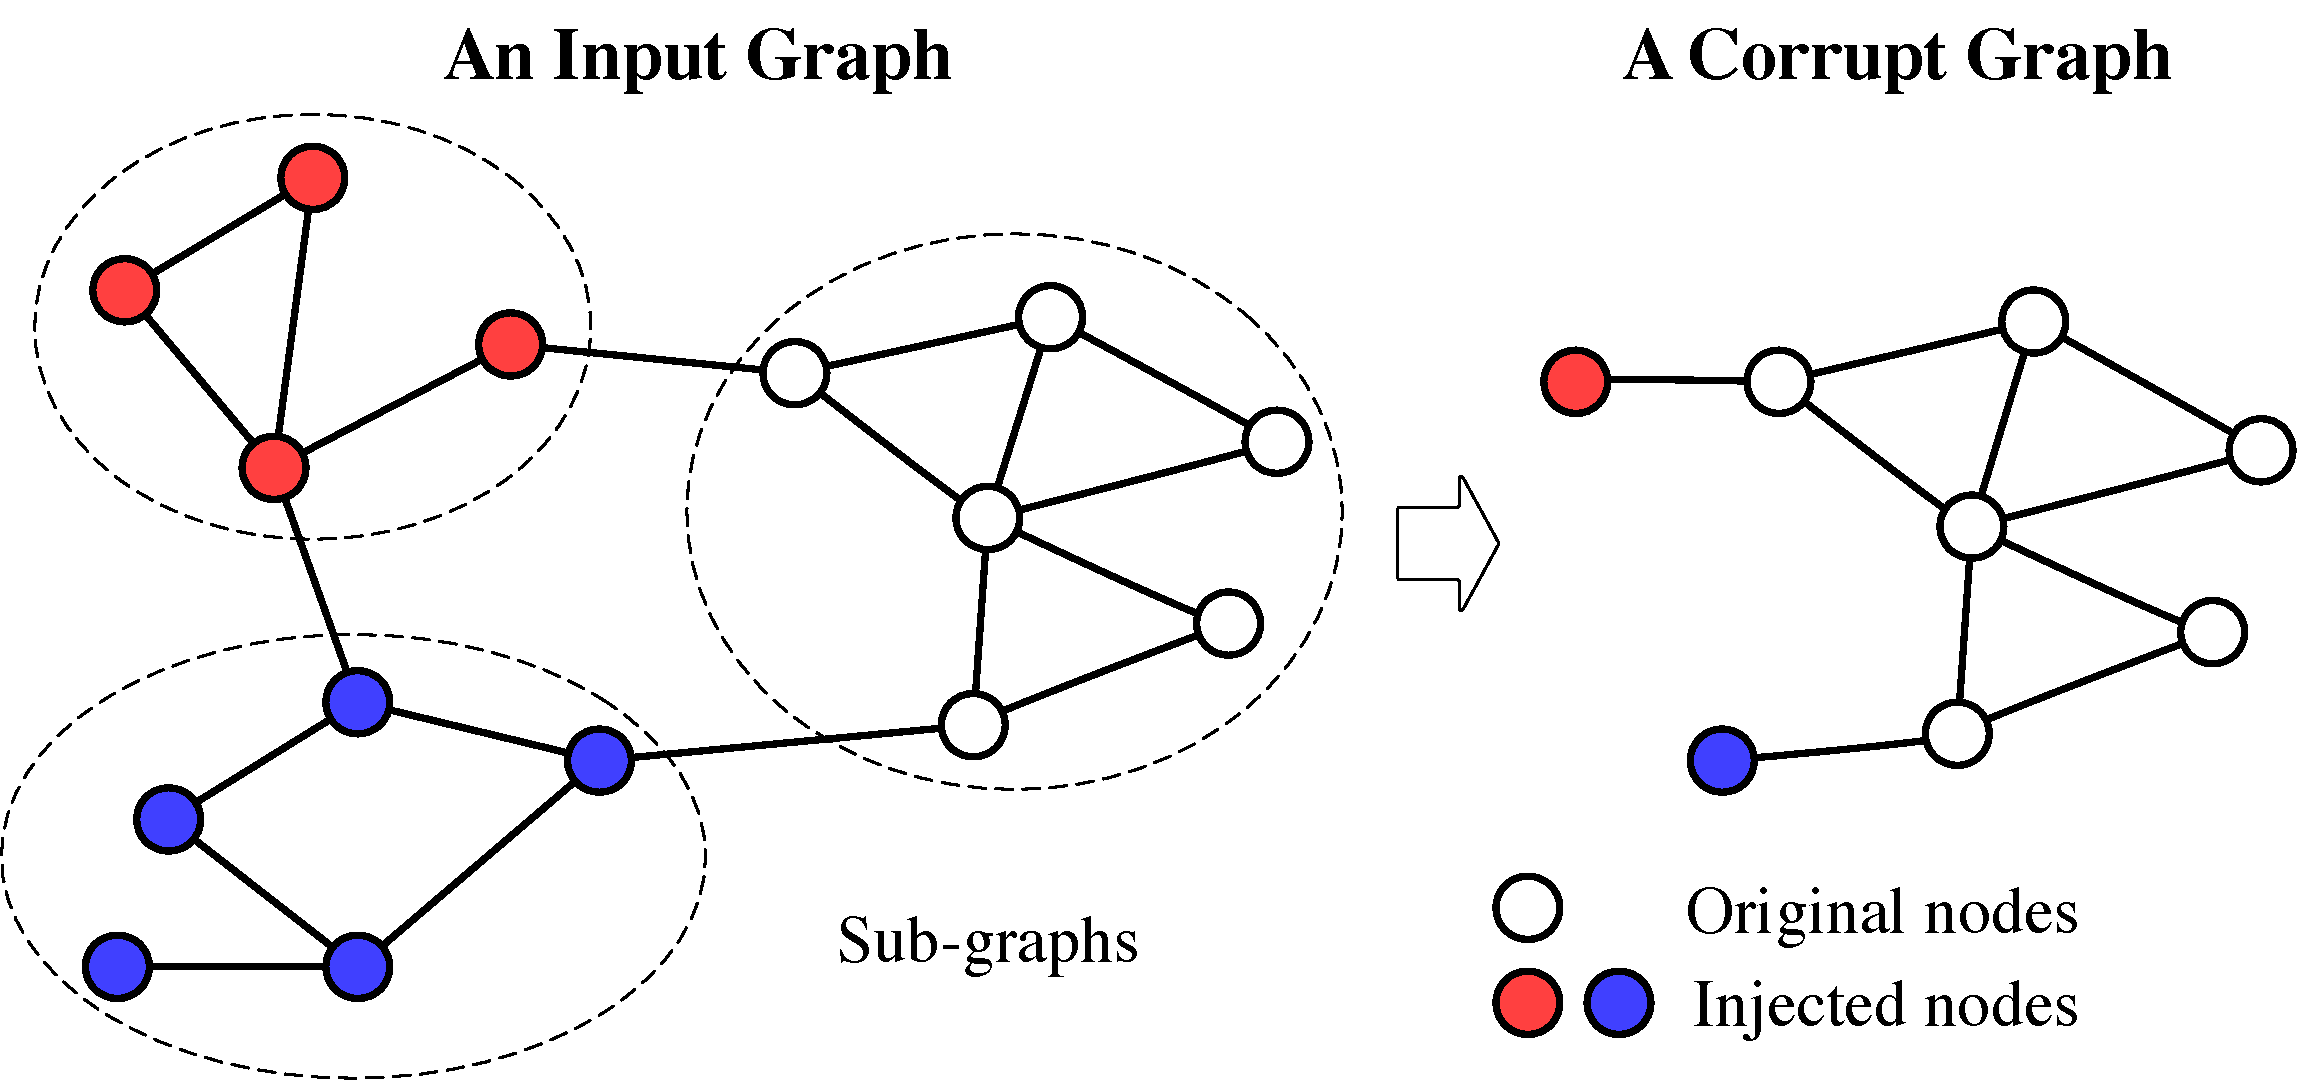
\includegraphics[width=0.46\textwidth]{figures/corrupt}
	\caption{\label{fig:corrupt} Illustration of constructing a corrupt graph.}
\end{figure}
Sufficient labels of the anomalies are often expensive to be obtained. For example, in AMiner\footnote{http://aminer.org}, an online academic system, it usually spends up to several hours to correct the collected papers for a top expert by a skilled annotator. And for annotating the fraudsters on business websites, the labeling criteria on abnormal behaviors is hard to be offered. Such scarce labels drives us to extend \smodel in an unsupervised manner.
Although a few GNN pre-training schemes in the unsupervised manner have been proved to be useful for the downstream node classification task~\cite{GAE, Graphsage}, anomaly detection, which pays more attention on a node's deviation from the majority instead of the node feature itself, is not exactly the same as node classification.

We propose a new pre-training scheme, \pmodel, to focus on tackling the anomaly detection problem. The basic idea is to construct pseudo labels via corrupting the original graph by injecting the nodes outside the graph as the anomalies and then pre-train \smodel on the corrupt graphs. The underlying assumption is nodes in different graphs follow  different feature distribution. A corrupt graph is defined as follows:

\begin{definition}
	\label{eq:corrupt_graph}
	\textbf{Corrupt Graph.} Given a set of homogenous graphs $\mathcal{G} = \{G_i\}_{i=1}^{M}$, we create an additional adjacency matrix $\mathcal{A}$ between the nodes in all the graphs, where the intra links are from individual graphs and the inter links are created by the same way as the intra links. For each graph $G_i=(V_i,A_i)$, we create a corrupt graph $\tilde{G}_i$ by injecting a set of nodes $\bar{V}_i $ from the graphs except $G_i$, i.e., $\bar{V}_i = \{v_j \in \mathcal{G} \setminus  G_i \}$, thus the corrupt nodes $\tilde{V}_i$ are the union of $V_i$ and $\bar{V}_i$, i.e., $\tilde{V}_i = V_i \cup \bar{V}_i$. The corrupt adjacency matrix is obtained by slicing $\mathcal{A}$ using the indexes in $\tilde{V}_i$. 
	%We mark $\mathcal{V}^+$ to denote the original node set $\{v^+_1, v^+_2, ..., v^+_N\}$. We then inject $\mathcal{M}$ ($\mathcal{M} \ll \mathcal{N}$) noisy nodes from other graphs, dented as $\mathcal{V}^-$, such that we obtain a corrupt graph $\mathcal{G}^{'} = \{\mathcal{V}^{'}, \boldsymbol{ \mathcal{X}^{'}}, \boldsymbol{\mathcal{A^{'}}}, \mathcal{Y}^{'}\}$, where $\mathcal{V}^{'} = \{v^+_1, ..., v^+_N, v^-_1, ..., v^-_M\}$, $\boldsymbol{ \mathcal{X}^{'}}, \boldsymbol{\mathcal{A^{'}}}$ are the corresponding feature and adjacency matrix, $\mathcal{Y}_i = 0$ if $i\in \left[1,\mathcal{N}\right]$ and $\mathcal{Y}_i = 1$ if $i\in \left(\mathcal{N}, \mathcal{N}+\mathcal{M}\right]$. 
\end{definition}


%Specifically, suppose we have collected multiple clean graphs, for each graph, we randomly sample several nodes from other graphs into it as the abnormal nodes and link them to the normal nodes in the original graph by the same criteria of creating the original links. 
For example, suppose we have collected paper networks of multiple researchers, for each researcher, we inject the wrong papers from others into his paper network as the abnormal nodes, and link them to the right papers if they share the same coauthor names. \figref{fig:corrupt} illustrates the process of creating a corrupt graph. 

For the scenario of a single network, we first cluster the nodes into multiple sub-graphs, and then construct the pseudo labels by the same way. For example, we cluster a user-rating-product network into multiple sub-graphs. For each sub-graph, we inject the nodes from other sub-graphs into it as the abnormal nodes, and link them with the normal nodes by the original user-rating-product relationships in the whole graph. 
The assumption is users favoring different products can be treated as anomalies with each other. We perform hierarchical agglomerative clustering algorithm (HAC) to cluster the nodes based on the initial features $X$ and determine the number of the clusters via finding the elbow point of Silhouette Coefficient~\cite{rousseeuw1987silhouettes}, a well-adopted clustering metric. 
%We conduct eigen-decomposition on the graph Laplacian s.t. $I-D^{-1/2}AD^{-1/2} = U\Lambda U^\top$ where $I$ is the identity matrix, $D$ is the degree matrix, use the top eigenvectors in U~\cite{von2007tutorial} as the features for each node, and then perform hierarchical agglomerative clustering algorithm (HAC) on the node features. 


On the corrupt graphs, we can optimize the same context-aware graph contrastive loss function defined in Eq.\eqref{eq:loss} to train $f_{\text{GNN}}$, which can be further fine-tuned on the target graph if the ground-true labels are available. 

\vpara{Connections with Other Graph Pre-training Frameworks.}
Existing graph pre-training frameworks helps less on anomaly detection. For example,  GAE~\cite{GAE} and GraphSAGE~\cite{Graphsage} reconstuct the adjacency matrix under the node proximity assumption, which is violated by the linkages between normal and abnormal nodes. 
GCC~\cite{qiu2020gcc} maximizes the consistency between the sampled ego-networks of a same node compared with those sampled from different nodes, such feature consistency assumption cannot explicitly help distinguish the abnormal nodes from the normal nodes. 
Although DGI~\cite{velickovic2019deep}, that contrasts a node with the whole graph, is similar to the contrastive objective function of \pmodel, the negative instances are addressed differently. In DGI, given a graph as the context, before contrasting, the positive nodes and negative nodes are convolved and represented in independent graphs. But in \pmodel, the negative nodes sampled from other graphs are injected and linked to the normal nodes in the concerned graph, which increases the difficulty of distinguishing the normal and abnormal nodes during training and improves the discrimination ability of the model. Essentially, DGI focuses more on representing the normal pattern while \spmodel additionally reinforce the differences of the abnormal nodes from the normal pattern.
%Under the circumstance, benign nodes are those from original graph, yet anomaly nodes are the ones from other different graphs. Hence we can also following the optimization methods motivated by the task of instance discrimination~\cite{wu2018unsupervised} that contrasts the benign nodes and the anomaly nodes from the graph context in an unsupervised contrastive learning manner. The infoNCE loss function~\cite{oord2018representation} is the same as the one defined in section.x.



\subsection{Anomaly Prediction}
For node $v_i \in G$ to be predicted, we get its embedding $\boldsymbol{h}_i^{(L)}$ and the graph embedding $\boldsymbol{q}^{(L)}$ of the final layer, and compute the cosine similarity between them as the abnormal extent of $v_i$. 


}